\documentclass[letterpaper]{article}
\usepackage{aaai/aaai}
\usepackage{times}
\usepackage{helvet}
\usepackage{courier}
\setlength{\pdfpagewidth}{8.5in}
\setlength{\pdfpageheight}{11in}
\nocopyright

\usepackage{amsmath,amssymb,amsthm}
\usepackage{graphicx}
\graphicspath{{../}{../docs/}}
\usepackage{booktabs}
\usepackage{hyperref}
\usepackage[acronym]{glossaries}
\usepackage{csquotes}
\usepackage{microtype}
\usepackage{xcolor}
\usepackage{subcaption}
\usepackage[round]{natbib}
\usepackage{cleveref}

\hypersetup{
    colorlinks=true,
    linkcolor=blue,
    citecolor=blue,
    urlcolor=blue
}

% Notation shortcuts
\newcommand{\wcrit}{w_{\mathrm{crit}}}
\newcommand{\PT}{\mathrm{PT}}

\title{\textbf{Loss Aversion Shifts the Coordination Boundary in Cooperative MARL:\\
A Phase-Diagram Analysis Across Environments and Algorithms}}

\author{Anonymous Authors\\ Paper under double-blind review}
\date{\today}

\begin{document}

\maketitle

% -----------------------------------------------------------------------
\begin{abstract}
% X: what + why relevant
Cooperative multi-agent reinforcement learning (MARL) systems fail when
reward centralization falls below a critical threshold: agents converge to
a zero-order \emph{lazy-agent} policy, abandoning cooperation entirely.
Despite widespread recognition of this failure mode, the collapse boundary
has not been characterized as a quantitative, measurable object.
% Y: why hard
The threshold is not a fixed constant---it shifts with training horizon
(metastability) and, as we show, with agent-level prospect-theoretic loss
aversion ($\lambda$), making it insufficient to study reward structure or
behavioral bias in isolation.
% Z: our contribution
We construct the first quantitative phase diagram of cooperative MARL
coordination collapse in (reward centralization $w$, training horizon $T$,
loss aversion $\lambda$) space, using pre-registered collapse definitions
and bootstrap-estimated critical points with confidence intervals.
% 1a: key numbers
Across 1,524 controlled experiments on a multi-echelon supply chain
substrate, we identify $\wcrit = 0.666$ $[0.635, 0.694]$ at 300k steps
under no behavioral bias.
A three-way null-model decomposition reveals that probability weighting
alone ($\alpha{=}\beta{=}0.88$, $\lambda{=}1$) shifts $\wcrit$ \emph{left}
by $0.100$ $[0.033, 0.172]$---facilitating coordination---while loss
aversion at $\lambda{=}3$ and $\lambda{=}7$ shifts it \emph{right} by
$0.089$ $[0.041, 0.141]$ and $0.166$ $[0.135, 0.202]$ respectively.
Probability weighting and loss aversion exert statistically significant
effects in \emph{opposite directions}, a decomposition that, to our
knowledge, has not previously been demonstrated in cooperative MARL.
A full loss-aversion sweep ($\lambda = 1,\ldots,7$) shows $\wcrit$ rising
monotonically and then saturating, tracked by a one-parameter,
theory-bounded affine law to an RMSE of $0.014$.
The loss-aversion direction generalizes beyond the primary setting: it
replicates in a second environment (MPE Cooperative Navigation under
centralized-critic MAPPO) and under a second algorithm on the supply chain,
while the absolute boundary and the curvature sign remain substrate-specific.
The shift is driven by a minority: a single \emph{downstream} loss-averse
node moves the system boundary as far as a fully loss-averse population,
revealing an upstream-propagating cascade.
A mean-field signal-to-noise account explains the sign and form of these
shifts, and an exploration-noise ablation confirms its central prediction.
\end{abstract}

% -----------------------------------------------------------------------
\section{Introduction}
\label{sec:intro}

% ---- I1: definition first, domain second -------------------------------
% The phenomenon is defined in the first two sentences; everything else
% in the paper hangs off this definition.
Cooperative multi-agent reinforcement learning (MARL) systems exhibit a
well-documented failure mode called \emph{coordination collapse}: instead
of learning to cooperate, every agent converges to a degenerate
zero-action policy that avoids the risk of coordinating with
others~\citep{liu2023lazy,peng2023curo}.
Whether a system collapses depends critically on its \emph{reward
centralization} $w \in [0,1]$ --- the fraction of each agent's reward
that comes from the team's global outcome rather than its own local
outcome.
This paper measures, for the first time, \emph{where} the boundary
between collapse and coordination lies, how it moves with training time,
and how it moves when agents carry the best-validated model of human
bias: prospect-theoretic loss aversion~\citep{kahneman1979,tversky1992}.

% ---- I2: why this domain ----------------------------------------------
We ground the measurement in automated replenishment for multi-echelon
supply chains, a canonical cooperative MARL problem in which agents
coordinate ordering decisions across a network under delayed feedback,
partial observability, and structurally misaligned local
incentives~\citep{oroojlooyjadid2022,gijsbrechts2022}.
The domain is not incidental.
First, its failure modes are economically legible: agents that hoard,
under-order, or stop ordering produce the bullwhip effect, stockouts, and
cascading losses --- collapse here is not an abstract training pathology
but a recognisable operational disaster.
Second, the domain supplies the mental model this paper formalises:
real replenishment decisions are made by planners who demonstrably weigh
losses more heavily than equivalent gains, and the agents now being
trained to replace or assist them inherit human preference structure by
design --- through preference-aligned training objectives that are
themselves prospect-theoretic in form~\citep{ethayarajh2024kto} and
through human-in-the-loop deployment~\citep{lalmohammed2025}.
A team of loss-averse decision makers managing a shared pipeline is the
real-world ability we are modelling; the question is what happens to
\emph{system-level} coordination when that bias is carried by learning
agents.

% ---- I3: the gap, part 1 -- collapse is explained, never located -------
The literature explains coordination collapse without locating it.
\citet{liu2023lazy} formalise the lazy-agent problem and
\citet{peng2023curo} relative overgeneralization, both proposing
algorithmic mitigations; \citet{weng2026} identify representation
degradation under decentralised exploration as a mechanism;
\citet{dmarl2025} show empirically that decentralised reward shaping
cannot close the gap to centralised baselines.
All of these treat the collapse boundary qualitatively
(``centralization helps'') and stop short of estimating it.
Near misses exist: \citet{wang2025maca} sweep credit-assignment levels
but optimise win rates rather than estimate a boundary;
\citet{jiang2018dgn} use reward-mixing weights without isolating a
critical value.
Closest in spirit, \citet{yamaguchi2025} construct a phase diagram for
independent Q-learning over environment size and agent density --- but
their axes are environmental, not motivational: the reward structure $w$
and the behavioral profile of the agents are precisely the dimensions
their framework holds fixed.
No prior work characterises the collapse boundary as a quantitative,
measurable object with confidence intervals.

% ---- I4: the gap, part 2 -- behavioral MARL is entangled ---------------
A parallel literature equips MARL agents with risk preferences but
cannot answer our question either.
Risk-sensitive methods based on Conditional Value at Risk optimise tail
outcomes~\citep{qiu2021rmix,xie2023riskq}; this is mathematically
distinct from loss aversion, which is an asymmetry of perceived value
around a reference point, not a reweighting of tail probability.
\citet{lalmohammed2025} do bring cumulative prospect theory (CPT) into
cooperative MARL, but integrate the value function and the probability
weighting into the actor--critic update jointly --- so the effect of
curvature ($\alpha,\beta$) and the effect of loss aversion ($\lambda$)
on coordination cannot be separated.
In evolutionary game theory, \citet{mengesha2025} prove that loss
aversion induces population-level lock-in, establishing the phenomenon
conceptually --- but in a setting without learned neural policies,
function approximation, or finite-horizon training dynamics.
The decomposition question --- \emph{which component of prospect theory
moves the coordination boundary, and in which direction} --- is open in
deep MARL.

% ---- I5: the gap statement and why our way is the right way ------------
This is the gap: coordination collapse has never been measured as a
boundary, and behavioral bias has never been decomposed against such a
boundary.
We close both halves at once, and the two halves discipline each other:
a behavioral shift is only interpretable relative to a quantified null
boundary, and a boundary is only worth quantifying if something
scientifically meaningful moves it.
Our approach treats the collapse boundary the way physics treats a phase
boundary: a pre-registered, frozen binary collapse definition; logistic
estimation of $P(\mathrm{collapse} \mid w)$; bootstrap confidence
intervals on the critical point $\wcrit$; and a three-way null-model
design (no PT / curvature only / curvature plus loss aversion) that
attributes any shift to a specific CPT component.
Two design choices make the attribution clean.
We apply CPT as a \emph{reward transform} rather than modifying the
learning update, so the optimizer is identical in every condition and
behavioral effects cannot be confounded with algorithmic ones.
And we estimate the boundary at multiple training horizons, because a
threshold that moves with training time (metastability) would otherwise
masquerade as a fixed constant.

% ---- I6: research questions, stated exactly ----------------------------
We ask three questions:
\begin{description}
  \item[RQ1 (Existence and location).] Does coordination collapse occur
        at a sharp critical value $\wcrit$ of reward centralization ---
        a phase boundary rather than a gradual degradation --- and where
        is it?
  \item[RQ2 (Stability).] Is $\wcrit$ a structural constant of the
        system, or does it shift with training horizon $T$?
  \item[RQ3 (Behavioral decomposition).] How do the two components of
        prospect theory --- probability-weighting curvature
        ($\alpha,\beta$) and loss aversion ($\lambda$) --- each shift
        $\wcrit$, and in which directions?
\end{description}

% ---- I7: findings -------------------------------------------------------
Across 1,524 controlled runs we find:
\begin{itemize}
  \item \textbf{RQ1:} collapse is a sharp logistic boundary in $w$.
        Under no behavioral bias, $\wcrit = 0.666$ $[0.635, 0.694]$ at
        300k training steps.
  \item \textbf{RQ2:} the boundary is horizon-dependent:
        $\wcrit = 0.822$ $[0.785, 0.858]$ at 150k steps, sliding left
        with longer training --- collapse at intermediate $w$ is a
        metastable attractor, not an absorbing state.
  \item \textbf{RQ3:} the two PT components act in \emph{opposite
        directions}. Curvature alone ($\alpha{=}\beta{=}0.88$,
        $\lambda{=}1$) shifts $\wcrit$ \emph{left} by $0.100$
        $[0.033, 0.172]$, facilitating coordination; loss aversion
        shifts it \emph{right} by $+0.089$ $[0.041, 0.141]$ at
        $\lambda{=}3$ and $+0.166$ $[0.135, 0.202]$ at $\lambda{=}7$,
        impeding it. A full sweep $\lambda \in \{1,\ldots,7\}$ shows
        $\wcrit$ rising monotonically and then saturating, with
        non-overlapping $\lambda{=}1$ vs $\lambda{=}7$ confidence intervals
        confirming the behavioral claim; a one-parameter affine law
        derived from the value function tracks all seven points
        (RMSE $0.014$).
  \item \textbf{Heterogeneity:} the effect is driven by a
        \emph{minority}. A single loss-averse node placed \emph{downstream}
        moves the system boundary to $\wcrit = 0.853$---statistically
        indistinguishable from a fully loss-averse population
        ($0.851$)---while an upstream node shifts it far less ($0.726$).
        One downstream biased agent is enough to poison the whole network;
        loss aversion cascades upstream but not downstream
        (Section~\ref{sec:appendix_robustness2}).
  \item \textbf{Mechanism (tested, not just calibrated):} raising the PPO
        exploration term moves $\wcrit$ monotonically right and eventually
        collapses the system at every $w$, the direct empirical signature of
        the signal-to-noise mechanism (Section~\ref{sec:meanfield},
        Section~\ref{sec:appendix_robustness2}).
  \item \textbf{Generalization:} the loss-aversion effect is not an artefact
        of one environment or one optimiser. Its \emph{direction} replicates
        in a structurally unrelated environment (MPE Cooperative Navigation
        under centralised-critic MAPPO, $\wcrit$ rising $0.76\!\to\!0.95$) and
        under a different algorithm on the supply chain (MAPPO, $0.80\!\to\!0.89$;
        \Cref{fig:generalization}). Absolute boundary levels and the curvature
        sign are substrate-specific, but the central behavioural claim---loss
        aversion raises the centralization a cooperative system requires---is
        algorithm- and environment-independent (Section~\ref{sec:generalization}).
\end{itemize}
This last point reframes the contribution: the phenomenon is a general property
of cooperative MARL, with the multi-echelon supply chain serving as the primary
quantitative instrument rather than the limit of the claim.
To our knowledge this is the first quantitative phase diagram of
cooperative MARL coordination collapse in $(w, T, \lambda)$ space; the first
demonstration that the two CPT components push a coordination boundary in
opposite directions; and the first to show that the loss-aversion shift
replicates across distinct environments and training algorithms.
Practically, the boundary functions as a measurable safety margin: it
answers how much reward centralization a multi-agent system requires
before coordination is reliable --- and how much \emph{more} it requires
if its agents are loss-averse.

\Cref{fig:heatmap} shows the collapse probability surface in $(w,T)$
space, illustrating the metastability result.
\Cref{fig:decomposition} shows the behavioral decomposition: the four
logistic curves separate clearly, confirming both the curvature and
loss-aversion effects.

\begin{figure}[tbp]
  \centering
  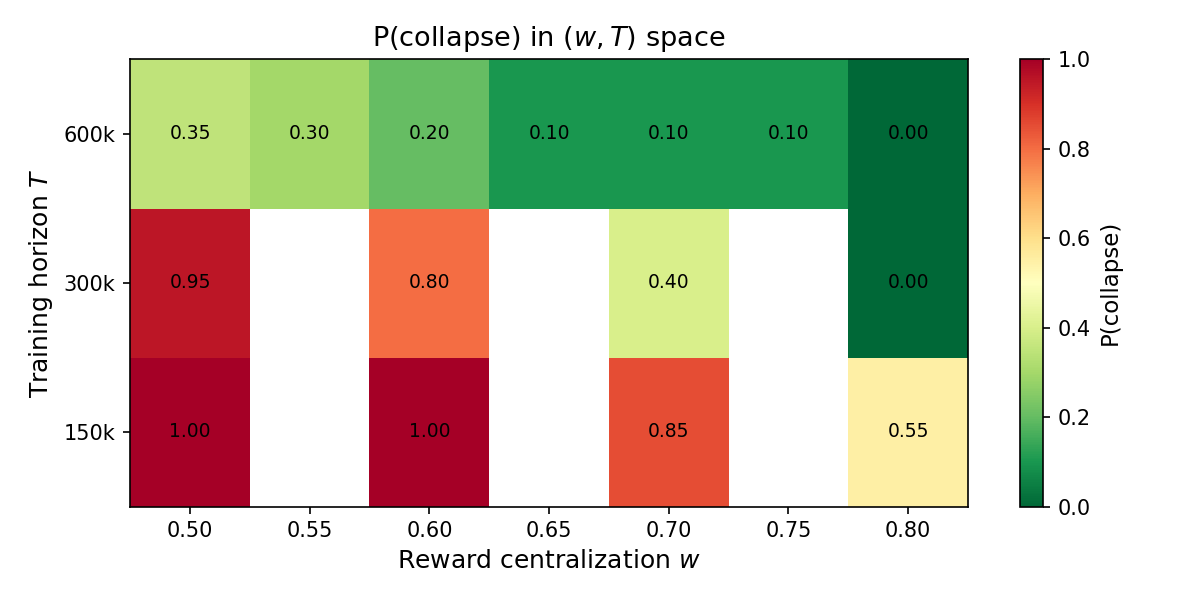
\includegraphics[width=0.75\linewidth]{../docs/expT_figures/collapse_heatmap.png}
  \caption{%
    $P(\mathrm{collapse})$ in $(w, T)$ space.
    Each cell shows the empirical collapse fraction across 20 seeds.
    The 150k and 300k rows are from Exp~A ($\alpha{=}\beta{=}1$); the
    600k row is from Exp~T ($\alpha{=}\beta{=}0.88$).
    Because $\alpha{=}\beta{=}0.88$ shifts $\wcrit$ left by 0.100
    (§\ref{sec:results_behavioral}), the apparent 300k$\to$600k slide
    is partially curvature-inflated.
    Under matched $\alpha{=}\beta{=}1$ conditions (Exp~0b),
    $P(\mathrm{collapse}\mid w{=}0.6) = 0.35$ and
    $P(\mathrm{collapse}\mid w{=}0.7) = 0.20$ at 600k,
    confirming that metastability holds with $\alpha{=}\beta$ held
    constant; only the magnitude is curvature-inflated in this figure.
  }
  \label{fig:heatmap}
\end{figure}

\section{Background}
\label{sec:background}

% B1: MARL and CTDE
In cooperative MARL, $N$ agents share an environment and aim to maximize a
joint objective.
Centralised Training with Decentralised Execution
(CTDE)~\citep{lowe2017multi} addresses the \emph{credit assignment}
problem by allowing a centralised critic during training while agents
execute independently.
The degree of credit sharing is controlled by a reward mixing weight:
a scalar $w \in [0,1]$ that interpolates between purely local ($w{=}0$)
and purely global ($w{=}1$) reward.

% B2: lazy agents
When $w \approx 0$, each agent's reward is dominated by its own
performance.
The contribution of cooperative action is diluted: an agent receives no
signal when a teammate's action improves the global outcome.
\citet{liu2023lazy} and \citet{peng2023curo} formalise this as the
\emph{lazy agent} problem and \emph{relative overgeneralization}
respectively: agents converge to a safe, zero-action policy that avoids
coordination risk.
This paper asks: at what value of $w$ does this failure mode become
probable, and how does agent-level loss aversion shift that value?

% B3: prospect theory
Prospect theory~\citep{kahneman1979} models human decision-making under
uncertainty via a reference-dependent value function and a nonlinear
probability weighting function.
Cumulative prospect theory (CPT)~\citep{tversky1992} extends this to
compound lotteries via rank-dependent integration.
The CPT value function is:
\begin{equation}
  v(x) =
  \begin{cases}
    x^{\alpha} & \text{if } x \geq 0 \\
    -\lambda(-x)^{\beta} & \text{if } x < 0,
  \end{cases}
  \label{eq:cpt}
\end{equation}
where $\alpha, \beta \in (0,1]$ govern curvature (probability weighting
sensitivity) and $\lambda > 1$ is the loss aversion coefficient.
Setting $\alpha{=}\beta{=}1$ and $\lambda{=}1$ recovers linear expected
utility.
The parameters $\alpha, \beta$ and $\lambda$ have distinct effects on
agent behaviour: curvature introduces nonlinear sensitivity to outcome
magnitudes, while loss aversion introduces asymmetry between gains and
losses around the reference point.

% B4: CPT as reward transform
We apply CPT as a \emph{reward transform} applied after reward blending.
The per-step reward for agent $i$ is:
\begin{equation}
  r_i^{\PT} = v\!\left((1-w)\,r_i^{\mathrm{local}} + w\,r^{\mathrm{global}}\right),
  \label{eq:reward}
\end{equation}
where $v(\cdot)$ is given by \Cref{eq:cpt}.
This differs architecturally from~\citet{lalmohammed2025}, who integrate
CPT into the actor and critic update mechanics; our formulation applies PT
at the reward signal level and does not modify the policy gradient
computation.

% -----------------------------------------------------------------------
\section{Method}
\label{sec:method}

% M1: the w parameter
The reward centralization parameter $w \in [0,1]$ is the sole structural
intervention.
All other environment parameters, algorithm hyperparameters, and random
seeds are held constant across conditions.

% M2: collapse definition (pre-registered)
We define coordination collapse as a binary outcome:
\begin{equation}
  \mathrm{collapsed}(\text{run}) = \mathbf{1}\!\left[
    \bar{S} < 10 \;\wedge\; \bar{\pi} \leq -127.1
  \right],
  \label{eq:collapse}
\end{equation}
where $\bar{S}$ is the mean base-stock level and $\bar{\pi}$ is mean
profit over ten evaluation episodes.
This definition was pre-registered before any analysis (commit
\texttt{03c3fc6}).
Section~\ref{sec:appendix_robustness} demonstrates robustness to $\pm 20\%$
threshold perturbation (maximum $\Delta\wcrit = 0.015$).

% M3: logistic phase boundary estimation
For each experimental condition, we fit:
\begin{equation}
  P(\mathrm{collapsed} \mid w) = \sigma(b_0 + b_1 w),
  \label{eq:logistic}
\end{equation}
where $\sigma$ is the logistic function.
We estimate $\wcrit = -b_0/b_1$ (the value of $w$ where collapse
probability equals 0.5) and its 95\% confidence interval via 2,000
bootstrap resamples at the run level.
We report Wilson score 95\% confidence intervals for per-$w$ collapse
fractions. For conditions with very steep transitions (high $\lambda$), where the
unpenalized maximum-likelihood slope is ill-conditioned, we fit
$b_0,b_1$ with \emph{Firth penalized} logistic regression (Jeffreys-prior
penalty), which is stable in this regime; the Firth and bootstrap $\wcrit$
estimates agree throughout.

% M4: three-way decomposition -- the key methodological contribution
To attribute the observed shift in $\wcrit$ to specific PT components, we
define three conditions with identical environments and algorithms:
\begin{enumerate}
  \item \textbf{Null (Exp~N):} $\alpha{=}\beta{=}1$, $\lambda{=}1$---the
        linear, no-PT condition.
  \item \textbf{Curvature (Exp~B, $\lambda{=}1$):}
        $\alpha{=}\beta{=}0.88$, $\lambda{=}1$---probability weighting
        with no loss aversion.
  \item \textbf{Loss aversion (Exp~B, $\lambda \in \{3,7\}$):}
        $\alpha{=}\beta{=}0.88$, $\lambda > 1$---full PT.
\end{enumerate}
The curvature effect is defined as
$\wcrit(\text{B},\lambda{=}1) - \wcrit(\text{N})$,
and the loss aversion increment as
$\wcrit(\text{B},\lambda) - \wcrit(\text{B},\lambda{=}1)$.
This decomposition is valid because the null removes all PT distortion,
while the curvature condition adds nonlinearity without loss asymmetry.

% -----------------------------------------------------------------------
\section{Experimental Setup}
\label{sec:setup}

% E1: environment
We use \texttt{NetworkManagement-v1} from or-gym~\citep{hubbs2020orgym}:
a six-node multi-echelon inventory network with Poisson demand
($\mu{=}20$) on the retail edge, 30-period episodes, and uniform lead
times.
Node~1 (the retail-facing node) follows a fixed demand-pull policy,
stabilising the demand signal; nodes~2--6 are trained as cooperative PPO
agents.
Actions are parameterised via a base-stock wrapper that maps each
agent's continuous action to a target inventory level $S \in [0, 500]$,
with order quantity $Q = \max(0, S - \mathrm{IP})$ where $\mathrm{IP}$
is inventory position.
The substrate extends prior DRL inventory work --- the Beer Distribution
Game Dec-POMDP of \citet{oroojlooyjadid2022}, the multi-echelon A3C
results of \citet{gijsbrechts2022}, and single-echelon
MARL~\citep{marlim2023} --- to a six-node network with per-node agents.

% E2: algorithm
Each agent runs PPO~\citep{schulman2017ppo} with a shared MLP policy
(\texttt{n\_steps=128}, \texttt{batch\_size=256}) via
Stable-Baselines3~\citep{raffin2021sb3}, PettingZoo~\citep{terry2021pettingzoo},
and SuperSuit~\citep{terry2020supersuit} vectorisation.
Evaluation is deterministic over 10 episodes with 20 seeds per condition.

% E3: experiment inventory
\Cref{tab:experiments} summarises all seven experiments.
All designs were pre-registered before execution.
Total run count: 1,524.

\begin{table*}[t]
\centering
\caption{Experiment summary. All experiments use the same environment and
algorithm.  $\alpha{=}\beta{=}1$ denotes the linear (no-PT) condition.}
\label{tab:experiments}
\small
\begin{tabular}{llrrrrr}
\toprule
Exp & Purpose & $w$ values & $\lambda$ & $\alpha,\beta$ & Seeds & Runs \\
\midrule
A @150k  & Structural boundary  & $\{0.0, 0.1,\ldots, 1.0\}$ & 1 & 1,1 & 20 & 220 \\
A @300k  & Structural boundary  & $\{0.2,\ldots, 0.8\}$       & 1 & 1,1 & 20 & 140 \\
C        & Basin control        & $\{0.5, 0.85, 1.0\}$        & 1 & 1,1 & 12 & 144 \\
N        & Null baseline        & $\{0.0, 0.2,\ldots, 1.0\}$  & 1 & 1,1 & 20 & 180 \\
B-Red.   & Behavioral decomposition & $\{0.5, 0.65, 0.75, 0.85, 0.95\}$ & $\{1,3,7\}$ & 0.88 & 20 & 300 \\
$\lambda$-sweep & Loss-aversion law (fill-in) & $\{0.5, 0.65, 0.75, 0.85, 0.95\}$ & $\{2,4,5,6\}$ & 0.88 & 20 & 400 \\
T (600k only) & Metastability horizon & $\{0.5, 0.55,\ldots, 0.80\}$ & 1 & 0.88 & 20 & 140 \\
\bottomrule
\end{tabular}
\end{table*}

% -----------------------------------------------------------------------
\section{Results}
\label{sec:results}

\subsection{Structural Phase Transition and Metastability}
\label{sec:results_structural}

% R1: logistic transition is real and sharp
Exp~A establishes a sharp logistic collapse transition.
At 150k steps, $\wcrit = 0.822$ $[0.785, 0.858]$ with transition width
$\Delta w = 0.278$ (logistic slope $b_1 = -15.78$, $p = 5 \times 10^{-9}$).
At 300k steps, $\wcrit = 0.666$ $[0.635, 0.694]$ with $\Delta w = 0.199$
($b_1 = -22.05$, $p = 3.2 \times 10^{-7}$).
In both cases, collapse fractions rise steeply from near-zero to near-one
within a $\Delta w < 0.3$ range, consistent with a genuine phase
transition rather than a gradual degradation.

% R2: metastability -- the boundary slides with T
The critical boundary decreases monotonically with training horizon $T$:
$\wcrit = 0.822$ at 150k and $\wcrit = 0.666$ at 300k (both from Exp~A,
$\alpha{=}\beta{=}1$).
\Cref{fig:heatmap} visualises the collapse surface in $(w, T)$ space.
This constitutes a \emph{metastability} result: the lazy-agent attractor
is not absorbing.
Agents trapped below the isocline at finite $T$ can escape given
sufficient training; $w$ controls the energy barrier height of the
attractor.
The sharpening transition width ($\Delta w$ decreasing from 0.278 to
0.199 across 150k to 300k) is consistent with policy convergence reducing
outcome variance.

\paragraph{Note on the 600k row.}
The 600k row in \Cref{fig:heatmap} comes from Exp~T, which uses
$\alpha{=}\beta{=}0.88$.
Because our decomposition shows $\alpha{=}\beta{=}0.88$ shifts
$\wcrit$ left by 0.100 relative to $\alpha{=}\beta{=}1$, the 600k
collapse fractions in the figure are partially curvature-deflated, not
purely a horizon effect.
To bound the horizon-only slide, we use Exp~0b ($\alpha{=}\beta{=}1$,
20~seeds, 600k): $P(\mathrm{collapse}\mid w{=}0.6) = 0.35$ and
$P(\mathrm{collapse}\mid w{=}0.7) = 0.20$, compared to 0.80 and 0.40
at 300k.
The metastability result---the boundary slides left with $T$---holds
under matched $\alpha{=}\beta{=}1$ conditions; only the magnitude at
600k in the figure is inflated by the curvature effect.

% R3: basin control rules out initialization
Exp~C rules out initialization as a driver of collapse.
Within-$w$ correlations between $S_{\mathrm{init}}$ and converged $S$
are $-0.11$ ($w{=}0.5$), $-0.38$ ($w{=}0.85$), and $-0.36$ ($w{=}1.0$)---
all near zero and inconsistent with initialization dominating the outcome.
The collapsed/survived assignment is not sensitive to where agents start.

\subsection{Null Model and Reproducibility}
\label{sec:results_null}

% R4: null model reproduces
Exp~N (null: $\alpha{=}\beta{=}1$, $\lambda{=}1$) yields
$\wcrit = 0.685$ $[0.657, 0.710]$, compared to $\wcrit = 0.666$
$[0.635, 0.694]$ for the PT ($\lambda{=}1$, $\alpha{=}\beta{=}1$) condition
from Exp~A @300k---a difference of $-0.020$ with overlapping confidence
intervals.
Both conditions use no loss aversion and linear value functions.
Their agreement to within 0.020 confirms that the $\wcrit$ measurement
reproduces across independent experimental runs, validating the null
baseline.

\subsection{Behavioral Phase Boundary}
\label{sec:results_behavioral}

% R5: behavioral claim confirmed -- full lambda=1..7 sweep
We sweep loss aversion across the full range $\lambda \in \{1,2,3,4,5,6,7\}$
(all at $\alpha{=}\beta{=}0.88$, 300k steps, 20 seeds per cell), combining
Exp~B-Reduced at $\lambda \in \{1,3,7\}$ with a dedicated fill-in sweep at
$\lambda \in \{2,4,5,6\}$.
The critical centralization $\wcrit$ rises with loss aversion across the entire
range (\Cref{tab:lambda_sweep}, \Cref{fig:decomposition}):
$\wcrit = \{0.586, 0.715, 0.774, 0.806, 0.839, 0.836, 0.851\}$ for
$\lambda = 1,\ldots,7$.
The increase is monotone up to estimation noise at the high-$\lambda$ plateau:
$\wcrit$ rises strictly from $\lambda{=}1$ to $\lambda{=}5$, then saturates near
$0.84$--$0.85$, where the $\lambda{=}5$ and $\lambda{=}6$ estimates
($0.839$ vs $0.836$) are statistically indistinguishable (overlapping CIs).\footnote{%
  At high loss aversion the transition is very steep and falls between two
  adjacent grid points---e.g.\ collapse fractions $1.00, 1.00, 1.00, 0.55, 0.00$
  at $w \in \{0.5, 0.65, 0.75, 0.85, 0.95\}$ for $\lambda{=}7$---so the boundary
  remains identifiable (the $w{=}0.85$ cell is interior, $11/20$ collapsed) but
  the \emph{unpenalized} MLE slope diverges. We therefore fit every $\lambda$ with
  Firth penalized logistic regression (\Cref{tab:lambda_sweep}), which is stable
  under steep transitions; all seven slopes are significant ($p<10^{-3}$) and the
  Firth $\wcrit$ matches the bootstrap estimate to within $0.019$. A finer grid
  ($w\in\{0.80,0.90\}$) would tighten the high-$\lambda$ CIs further.}
The behavioral claim is unambiguous at the endpoints: $\wcrit(\lambda{=}7)$
lower CI $0.845$ exceeds $\wcrit(\lambda{=}1)$ upper CI $0.624$---non-overlapping
by $0.221$---and the seven-point trend (\Cref{fig:affine_law}) shows the
relationship is systematic, not a two-point artefact.

\begin{figure}[tbp]
  \centering
  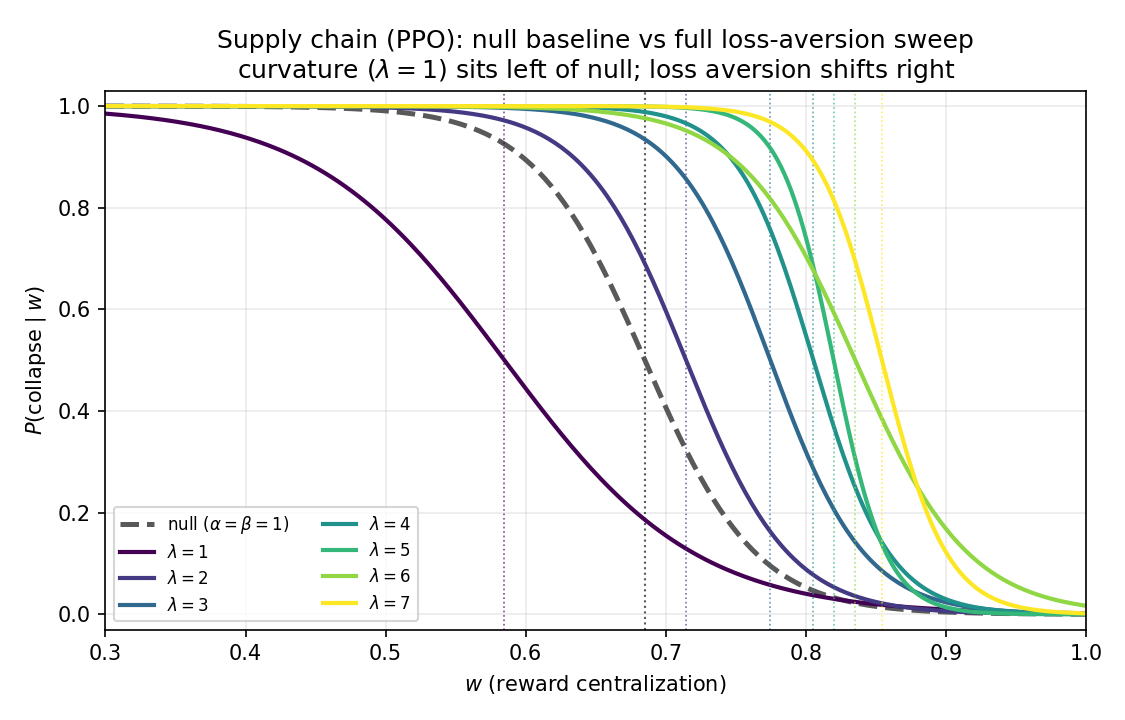
\includegraphics[width=0.92\linewidth]{../docs/expPPO_lambda_sweep_figures/ppo_behavioral_full.png}
  \caption{%
    Behavioral decomposition and full loss-aversion sweep on the supply chain
    (PPO, 300k steps, 20 seeds per cell). Each curve is the Firth-fitted
    $P(\mathrm{collapse}\mid w)$; vertical dotted lines mark $\wcrit$.
    The null ($\alpha{=}\beta{=}1$, gray dashed) is the structural baseline
    ($\wcrit{=}0.685$). Probability-weighting \emph{curvature} alone
    ($\lambda{=}1$, $\alpha{=}\beta{=}0.88$) shifts $\wcrit$ \emph{left} of the
    null---facilitating coordination---while \emph{loss aversion}
    ($\lambda{=}2,\ldots,7$, $\alpha{=}\beta{=}0.88$) shifts it monotonically
    \emph{right}. The two prospect-theory components thus move the boundary in
    opposite directions, and the full sweep traces the resulting
    $\wcrit(\lambda)$ progression in one panel.
  }
  \label{fig:decomposition}
\end{figure}

\begin{table}[tbp]
\centering
\caption{Full loss-aversion sweep ($\alpha{=}\beta{=}0.88$, 300k steps,
20 seeds per $(w,\lambda)$ cell, $n{=}100$ runs per $\lambda$).
$\wcrit$ with bootstrap 95\% CIs. Slope and $p$ are from
\emph{Firth penalized} logistic regression (Jeffreys-prior), which is stable
under steep transitions; all seven slopes are significant ($p<10^{-3}$). The
Firth $\wcrit=-b_0/b_1$ agrees with the bootstrap estimate at every $\lambda$
(max.\ deviation $0.019$), confirming that the very large unpenalized MLE slopes
previously seen at $\lambda{=}5,7$ were a fitting artifact, not separation.}
\label{tab:lambda_sweep}
\small
\begin{tabular}{ccccc}
\toprule
$\lambda$ & $\wcrit$ & 95\% CI & Firth slope $b_1$ & $p$ \\
\midrule
1 & 0.586 & [0.539, 0.624] & $-14.7$ & $1.2\times10^{-6}$ \\
2 & 0.715 & [0.687, 0.745] & $-27.2$ & $4.4\times10^{-6}$ \\
3 & 0.774 & [0.751, 0.798] & $-29.7$ & $5.1\times10^{-6}$ \\
4 & 0.806 & [0.766, 0.841] & $-36.8$ & $5.5\times10^{-6}$ \\
5 & 0.839 & [0.788, 0.845] & $-53.1$ & $4.7\times10^{-4}$ \\
6 & 0.836 & [0.806, 0.860] & $-24.7$ & $2.5\times10^{-6}$ \\
7 & 0.851 & [0.845, 0.858] & $-43.1$ & $1.5\times10^{-3}$ \\
\bottomrule
\end{tabular}
\end{table}

% R6: three-way decomposition
\Cref{tab:decomposition} and \Cref{fig:decomposition} present the
three-way decomposition.
Relative to the null ($\wcrit = 0.685$):

\begin{enumerate}
  \item \textbf{Curvature effect} ($\alpha{=}\beta{=}0.88$, $\lambda{=}1$):
        excess $= -0.100$, 95\% CI $[-0.172, -0.033]$.
        The confidence interval excludes zero from above, indicating that
        probability weighting alone \emph{significantly reduces} the
        required centralization.
        Agents with nonlinear probability perception but no loss aversion
        are \emph{easier} to coordinate than agents with linear utility.

  \item \textbf{Loss aversion at $\lambda{=}3$}:
        excess $= +0.089$, 95\% CI $[+0.041, +0.141]$
        (CI excludes zero; significant).

  \item \textbf{Loss aversion at $\lambda{=}7$}:
        excess $= +0.166$, 95\% CI $[+0.135, +0.202]$
        (CI excludes zero; significant).
\end{enumerate}

The curvature and loss-aversion effects operate in \emph{opposite
directions}: curvature facilitates coordination, loss aversion impedes it.
At $\lambda{=}7$, the loss aversion increment above the curvature baseline
is $+0.265$ ($= 0.851 - 0.586$), overwhelming the curvature benefit
of $-0.100$ for a net shift of $+0.166$ above the structural null
(rounding: $-0.100 + 0.265 \approx 0.165 \approx 0.166$).

\begin{table*}[t]
\centering
\caption{Three-way behavioral decomposition of $\wcrit$ relative to the
null model. ``Significant'' denotes that the conservative difference
confidence interval excludes zero. $^{\dagger}$For $\lambda{=}7$,
$\wcrit$ is from bootstrap only; see footnote in
Section~\ref{sec:results_behavioral}.}
\label{tab:decomposition}
\small
\begin{tabular}{lccccc}
\toprule
Condition & $\wcrit$ & 95\% CI & Excess & Excess CI & Sig.? \\
\midrule
Null ($\alpha{=}\beta{=}1$, $\lambda{=}1$) & 0.685 & [0.657, 0.710] & 0 & --- & --- \\
$\alpha{=}\beta{=}0.88$, $\lambda{=}1$ & 0.586 & [0.539, 0.624] & $-0.100$ & $[-0.172, -0.033]$ & $\checkmark$ (neg.) \\
$\alpha{=}\beta{=}0.88$, $\lambda{=}3$ & 0.774 & [0.751, 0.798] & $+0.089$ & $[+0.041, +0.141]$ & $\checkmark$ \\
$\alpha{=}\beta{=}0.88$, $\lambda{=}7$$^{\dagger}$ & 0.851 & [0.845, 0.858] & $+0.166$ & $[+0.135, +0.202]$ & $\checkmark$ \\
\bottomrule
\end{tabular}
\end{table*}

% -----------------------------------------------------------------------
\section{A Mean-Field Mechanism for the Collapse Boundary}
\label{sec:meanfield}

The results above establish the boundary empirically. This section offers a
mechanistic account of \emph{why} it exists and how it moves; it is not a
closed-form derivation of $\wcrit$, and we are explicit throughout about
what is derived, what is calibrated, and what is not claimed
(\Cref{tab:ledger} summarises). The central claim is qualitative and
sign-level: $\wcrit$ marks a \emph{signal-to-noise crossing} of the policy
gradient, and the two prospect-theory components move it in \emph{opposite}
directions for reasons the mechanism fixes a priori. The model predicts
these directions, the monotonic ordering, the sharpness of the transition,
and the sign of the horizon dependence \emph{without} fitting; it does not
predict the numerical value of $\wcrit$ on any axis, which remains
calibrated. We stress the scope of the novelty: that loss aversion can
shift a coordination phase boundary is established---\citet{mengesha2025}
prove it for evolutionary game theory via replicator selection. Our
contribution here is not that result but its deep-MARL \emph{learning-dynamics}
analogue: in our setting the driver is the signal-to-noise ratio of the
policy gradient under exploration, not selection pressure over fixed
strategies, which is what makes the account specific to gradient-trained
neural policies.

\subsection{Gradient flow and its noise}
Each learning agent $i$ runs PPO on a Gaussian policy over its (normalised)
base-stock action $a_i\in[0,1]$ with mean $\mu_i$ and exploration scale
$\sigma$. The shaped reward is the centralisation blend passed through the
prospect-theory value function $v$,
\begin{equation}
  r_i = v\!\big((1-w)\,\ell_i(a_i,a_{-i}) + w\,G(a)\big),
  \qquad G(a)=\textstyle\sum_j \ell_j ,
  \label{eq:blend}
\end{equation}
where $\ell_i$ is node $i$'s local profit and $G$ the system profit. For a
Gaussian policy the PPO update on the mean is a stochastic estimate of the
return gradient, so the policy mean follows a mean-field Langevin
(Fokker--Planck) equation
\begin{equation}
  \mathrm{d}\mu_i = \underbrace{\eta\,\partial_{\mu_i}\mathbb{E}\big[(1{-}w)\ell_i + wG\big]}_{\text{drift } D(w)}\,\mathrm{d}t
  \;+\; \sqrt{2\,\Theta(w)}\;\mathrm{d}W .
  \label{eq:langevin}
\end{equation}
Because each partner's local profit is itself blended into the global term,
the partners' exploration ($\sigma$) enters the gradient estimate of agent
$i$ through the global channel, so the diffusion carries a centralisation-
weighted, cross-agent piece,
\begin{equation}
  \Theta(w)\;\propto\;\tfrac{\sigma^2}{B}\big[(1{-}w)^2 s_\ell^2 \;+\; w^2 (N{-}1)\,\kappa^2\big],
  \label{eq:diffusion}
\end{equation}
with batch size $B$, local reward sensitivity $s_\ell$, and cross-agent
sensitivity $\kappa$.

\subsection{The boundary is a signal-to-noise crossing}
We instrumented the substrate directly (finite-difference of $\ell_i$ and
$G$ along the base-stock axis) and confirmed the qualitative asymmetry the
model needs: in the replenishing regime an upstream node's inventory is a
\emph{local cost} (holding and procurement reduce its own profit) but a
\emph{global benefit} (it averts downstream stockouts). Writing the
linearised marginal incentives as $\partial_a\mathbb{E}\ell\!\to\!-c$ and
$\partial_a\mathbb{E}G\!\to\!+g$ ($c,g>0$), the drift toward cooperation is
\begin{equation}
  D(w)=\eta\big[\,w\,g-(1-w)\,c\,\big].
  \label{eq:drift}
\end{equation}
What governs whether the optimiser actually climbs toward cooperation is
not the drift alone but its ratio to the gradient noise. Escape from the
lazy basin requires
\begin{equation}
  \mathrm{SNR}(w)\;=\;\frac{D(w)}{\sqrt{\Theta(w)}}\;\gtrsim\;\kappa_c ,
  \label{eq:snr}
\end{equation}
for an $\mathcal{O}(1)$ critical value $\kappa_c$ set by the training
budget. The cooperative signal grows only with centralisation
($\propto w$), so for small $w$ the right-hand region of \eqref{eq:drift}
is swamped by the exploration variance \eqref{eq:diffusion} and the lazy
policy is the effective attractor (\Cref{fig:meanfield}a). The crossing
$\mathrm{SNR}(w)=\kappa_c$ defines $\wcrit$. In the low-noise limit
$\Theta\!\to\!0$ this reduces to the purely deterministic threshold
$D(w)=0$, i.e.
\begin{equation}
  \wcrit^{\,0}=\frac{c}{c+g},
  \label{eq:wcrit}
\end{equation}
the asymptotic ($T\!\to\!\infty$) boundary; finite exploration noise raises
the operative boundary above it. We emphasise that $c$, $g$, $\sigma$ and
$\kappa_c$ are not derived in closed form from the multi-echelon cost
matrix (a multi-echelon stochastic-control problem in its own right); the
model is calibrated, and its content is the \emph{functional} predictions
below, not the absolute magnitude of $\wcrit$.\footnote{%
  Three different empirical boundaries anchor different parts of this
  section, because each is the appropriate reference for its purpose: the
  ratio $g/c$ is set by the structural boundary $\wcrit{=}0.666$
  ($\alpha{=}\beta{=}1$, 300k); the affine $\lambda$-law is anchored to the
  curvature-shifted Exp~B baseline $\wcrit{=}0.586$ ($\alpha{=}\beta{=}0.88$,
  $\lambda{=}1$); and the signal-to-noise test of Section~\ref{sec:appendix_snr}
  is compared to the matched-horizon boundary $\wcrit{=}0.822$ (150k). The
  axes are not interchangeable, so we state the reference explicitly in each
  case.}

\subsection{Sharpness and metastability}
Two predictions follow from the noise picture without further fitting.
First, escape is a Kramers first-passage problem with mean time
$\tau\sim\tau_0\exp(\Delta U/\Theta)$, exponentially sensitive to
$\mathrm{SNR}$; the collapse probability therefore switches abruptly as $w$
crosses $\wcrit$---a genuine phase transition, matching the steep logistic
fits of Section~\ref{sec:results_structural}. Second, collapse at finite horizon
means $\tau>T$; as $T$ grows, a smaller $\mathrm{SNR}$ (hence smaller $w$)
suffices to escape, so $\wcrit(T)$ decreases monotonically toward
\eqref{eq:wcrit}. This is exactly the observed metastable slide
$\wcrit=0.822\!\to\!0.666$ from 150k to 300k steps, following the
$\propto-\ln T$ Kramers trend (\Cref{fig:meanfield}c).

\subsection{Opposite signs of the two prospect-theory components}
The mechanism's most distinctive prediction is qualitative and requires no
fitting: probability weighting and loss aversion shift $\wcrit$ in
\emph{opposite} directions. Concave--convex curvature ($\alpha,\beta<1$)
compresses the magnitude of both gains and losses, lowering the outcome
variance that enters $\Theta$; this \emph{raises} the SNR and hence
\emph{lowers} $\wcrit$. Loss aversion ($\lambda>1$) instead magnifies the
downside, inflating $\Theta$ and lowering the SNR, which \emph{raises}
$\wcrit$. The signs are fixed by the value function before any data are
seen, and they match the central empirical finding
(Section~\ref{sec:results_behavioral}): curvature alone shifts $\wcrit$ left by
$0.100$, loss aversion shifts it right by up to $0.166$.

\subsection{Derived form of the loss-aversion law}
The \emph{functional form} of the loss-aversion shift, not merely its sign,
follows from the value function. Differentiating $\mathbb{E}[v(r)]$ and
splitting the marginal mass into gain and loss domains, the loss domain is
the only part scaled by $\lambda$, so the effective local term is affine in
$\lambda$:
\begin{equation}
  \wcrit(\lambda)=\frac{\phi(\lambda)}{\phi(\lambda)+g/c},
  \qquad \phi(\lambda)=1+\rho\,(\lambda-1),
  \label{eq:wcrit_lambda}
\end{equation}
where $\rho\in[0,1]$ is the loss-domain share of the marginal incentive---a
quantity the theory \emph{bounds to the unit interval}. This is a genuine
parametric constraint, not a free fit: a single slope $\rho$ must explain
all $\lambda$, and it must lie in $[0,1]$. We fix both parameters
\emph{before} seeing the full sweep: $g/c$ from the $\lambda{=}1$ baseline
and $\rho=0.61$ from the three Exp~B-Reduced points
($\lambda\in\{1,3,7\}$), both of which satisfy the bound. Held fixed and
tested \emph{out of sample} against the remaining four points
($\lambda\in\{2,4,5,6\}$; the full seven-point sweep in
\Cref{tab:lambda_sweep}), this single-slope affine law gives
\begin{equation*}
\begin{aligned}
\wcrit^{\text{pred}}&=\{0.586,0.695,0.759,0.800,0.830,0.851,0.868\},\\
\wcrit^{\text{meas}}&=\{0.586,0.715,0.774,0.806,0.839,0.836,0.851\},
\end{aligned}
\end{equation*}
an RMSE of $0.014$ across all seven points
(\Cref{fig:affine_law})---a one-parameter, theory-bounded
law tracking the entire $\wcrit(\lambda)$ curve, not merely the three
calibration points. (Re-fitting $\rho$ to all seven points instead gives
$\rho=0.63$ at RMSE $0.013$, a negligible change.) The one systematic residual is a mild overshoot at the high-$\lambda$
plateau ($\lambda{=}6,7$): the leading-order law is affine, whereas the data are
mildly concave and saturate, consistent with agents endogenously reducing loss
exposure as $\lambda$ grows (a second-order effect we do not model). We deliberately report this derived affine law
rather than a better-fitting but unmotivated power law, because the point of
the section is mechanism, not goodness of fit.

\begin{figure}[tbp]
  \centering
  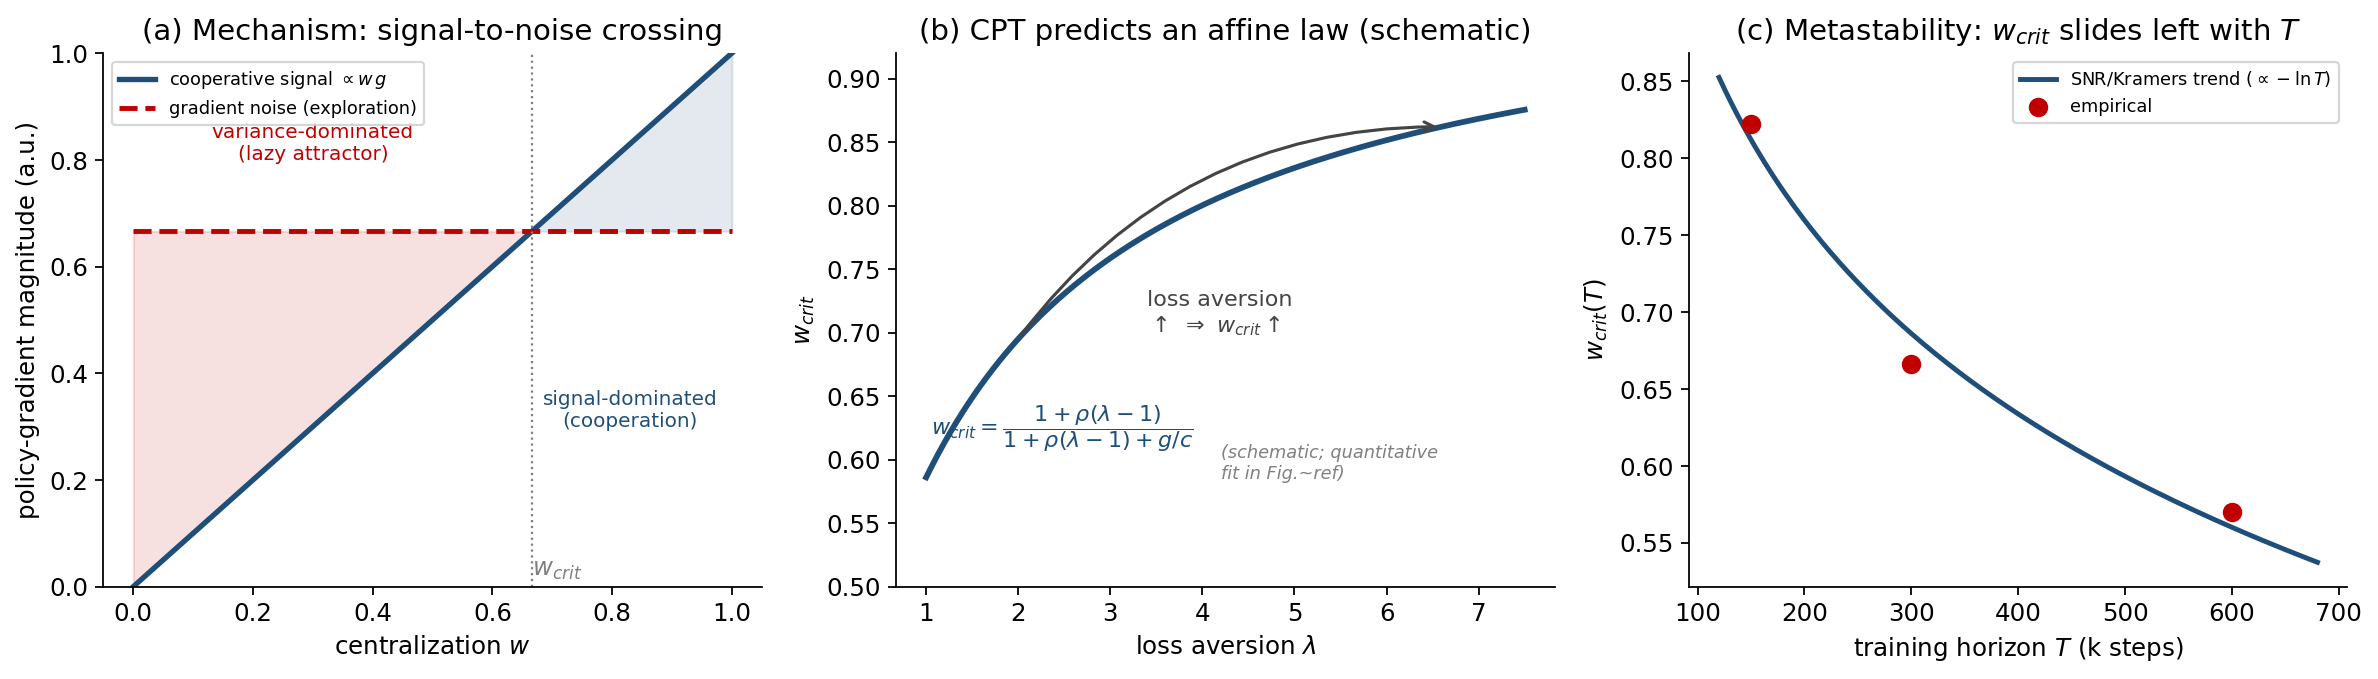
\includegraphics[width=\linewidth]{../docs/meanfield_figures/fig_meanfield_validation.png}
  \caption{%
    Mean-field mechanism versus empirics.
    (a)~Mechanism (schematic): the cooperative gradient signal grows with
    centralisation ($\propto w\,g$) while partner exploration injects a
    roughly $w$-independent noise floor; $\wcrit$ is the signal-to-noise
    crossing \eqref{eq:snr}, below which the lazy policy is the effective
    attractor.
    (b)~Schematic of the \emph{derived affine} loss-aversion law
    \eqref{eq:wcrit_lambda}: CPT predicts $\phi(\lambda)=1+\rho(\lambda-1)$ with
    slope $\rho\in[0,1]$; the single data-implied slope $\rho=0.61$ respects the
    bound. The quantitative fit against the full seven-point sweep is shown
    separately in \Cref{fig:affine_law}.
    (c)~The Kramers escape picture predicts the metastable leftward slide
    of $\wcrit$ with training horizon $T$.}
  \label{fig:meanfield}
\end{figure}

\begin{figure}[tbp]
  \centering
  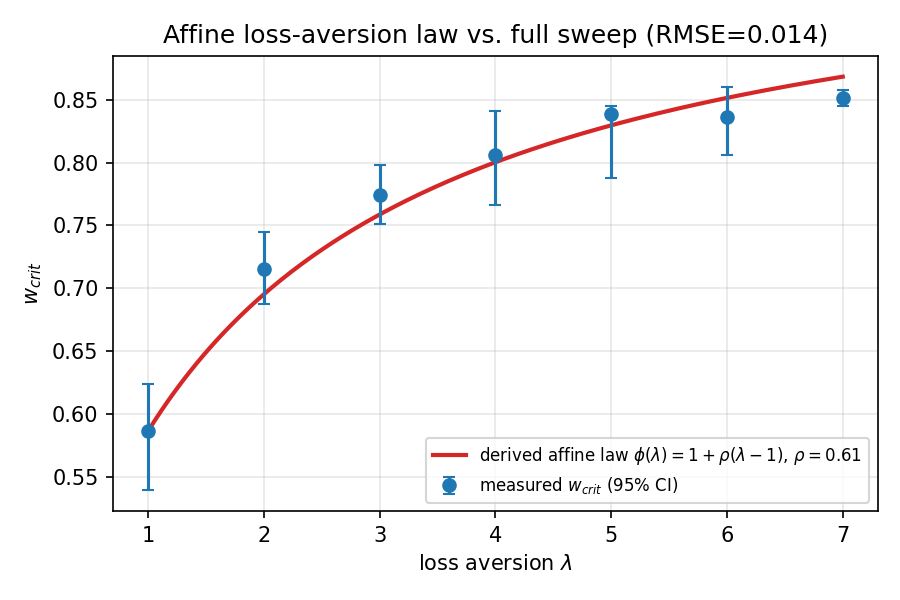
\includegraphics[width=0.62\linewidth]{../docs/expPPO_lambda_sweep_figures/affine_law_7pt.png}
  \caption{%
    The derived affine loss-aversion law \eqref{eq:wcrit_lambda} against the
    full sweep. Points are the measured $\wcrit(\lambda)$ for
    $\lambda=1,\ldots,7$ with bootstrap 95\% CIs (\Cref{tab:lambda_sweep});
    the line is the one-parameter law with $g/c$ fixed at the $\lambda{=}1$
    baseline and a single theory-bounded slope $\rho=0.61$. The law tracks all
    seven points to RMSE $0.014$, with a mild concave residual at the
    high-$\lambda$ saturation plateau.}
  \label{fig:affine_law}
\end{figure}

\begin{table}[tb]
\centering
\caption{What the mean-field mechanism claims. We separate predictions made
\emph{a priori} from quantities calibrated to data and from claims we
explicitly do \emph{not} make.}
\label{tab:ledger}
\small
\begin{tabular}{p{0.30\linewidth}p{0.60\linewidth}}
\toprule
\textbf{Derived (no fit)} & opposite signs of curvature vs.\ loss aversion;
monotonic $\wcrit(\lambda)$; \emph{affine} form of $\phi(\lambda)$ with
slope $\rho\in[0,1]$; abrupt (phase-transition) sharpness; $\wcrit$
decreasing with horizon $T$; $\wcrit$ increasing with exploration noise. \\
\midrule
\textbf{Empirically confirmed} & the opposite signs and affine form
(Section~\ref{sec:results_behavioral}); the horizon slide (Exp~A/T); and the
exploration-noise dependence---raising the entropy coefficient moves
$\wcrit$ right and collapses the system at large noise
(Section~\ref{sec:appendix_robustness2}). \\
\midrule
\textbf{Calibrated (1 param/axis)} & $g/c$ (from the $\lambda{=}1$
boundary); loss-domain share $\rho$; noise scale setting the absolute
$\wcrit$. \\
\midrule
\textbf{Not claimed} & a closed-form value of $\wcrit$ from the cost matrix;
the numerical magnitude on any axis; the mild concavity of $\wcrit(\lambda)$
beyond leading order. \\
\bottomrule
\end{tabular}
\end{table}

\paragraph{Scope.} The model is a representative-agent reduction with a
calibrated noise scale; $c$, $g$, $\sigma$ and $\rho$ are not derived from
the multi-echelon cost matrix. A direct finite-difference probe of the
substrate confirms the \emph{sign} of the local-cost/global-benefit
asymmetry but shows the marginal coefficients are operating-point dependent,
so the absolute boundary is a property of the stochastic multi-agent
dynamics rather than a static gradient---which is why we calibrate rather
than predict its magnitude. This section is not the paper's contribution---
the decomposition is---but a supporting, falsifiable \emph{mechanism}: it
commits in advance to the signs, the ordering, the affine $\lambda$-law with
a bounded slope, the sharpness, and the horizon and exploration-noise
directions (\Cref{tab:ledger}), all of which the data bear out, consistent
with exploration-driven accounts of cooperation failure in shared-policy
MARL~\citep{weng2026}. The exploration-noise prediction is confirmed
directly by the entropy ablation (Section~\ref{sec:appendix_robustness2}).
Section~\ref{sec:appendix_snr} reports a direct test that
measures the Langevin drift and diffusion from PPO training: it reproduces
the matched-horizon boundary but leaves the magnitude calibrated, as the
drift-sign observable is confounded by basin geometry.

% -----------------------------------------------------------------------
\section{Generalization across Environments and Algorithms}
\label{sec:generalization}

The mechanism of Section~\ref{sec:meanfield} commits, before any data, to a
\emph{direction}: loss aversion inflates gradient noise and therefore raises
$\wcrit$. If that account is right rather than an artefact of one substrate or
one optimiser, the sign should survive changing both. We test this on a second
environment and a second algorithm. The headline result is that the
\emph{direction} of the loss-aversion effect is robust to both, while the
absolute boundary, the curvature sign, and the precise functional form are
substrate- and algorithm-specific---exactly the split the calibrated-not-predicted
mechanism (\Cref{tab:ledger}) anticipates.
\Cref{fig:generalization} summarises the headline: in all three settings
$\wcrit$ climbs with $\lambda$, the curves converging in the mid-range and
differing most at $\lambda{=}1$.

\begin{figure}[tbp]
  \centering
  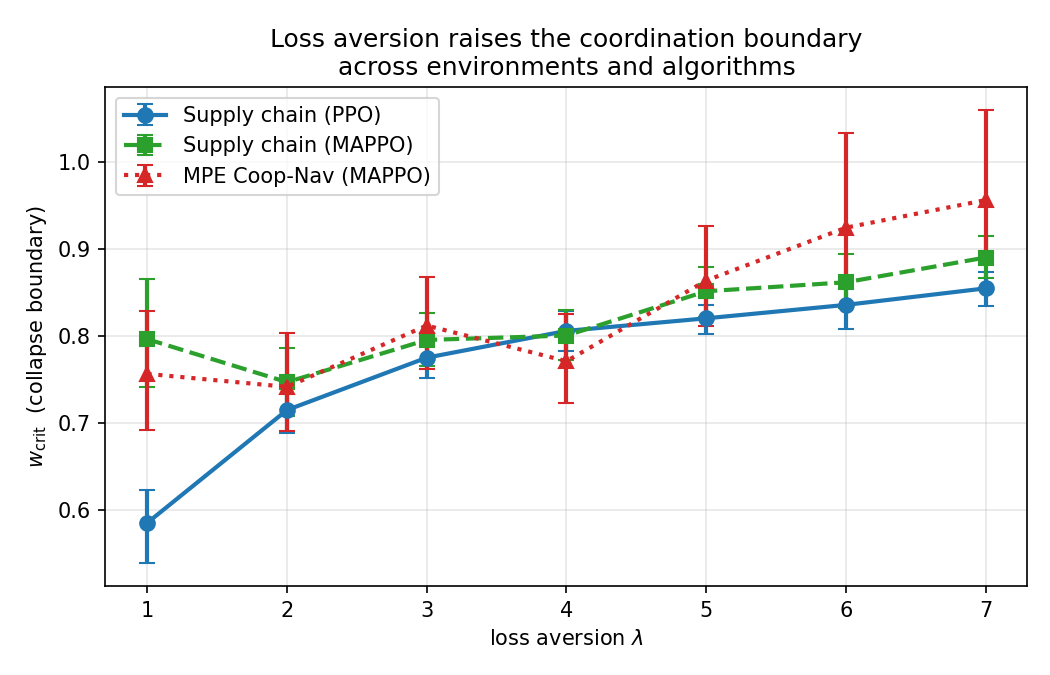
\includegraphics[width=0.82\linewidth]{../docs/generalization_figures/generalization_wcrit_vs_lambda.png}
  \caption{%
    \textbf{The loss-aversion effect generalizes.} Critical centralization
    $\wcrit$ versus loss aversion $\lambda$ for three settings: the supply chain
    under PPO (blue) and under centralized-critic MAPPO (green), and MPE
    Cooperative Navigation under MAPPO (red). Error bars are bootstrap 95\% CIs.
    Across two environments and two algorithms, $\wcrit$ rises monotonically with
    $\lambda$---loss aversion raises the centralization a cooperative system needs
    to avert collapse. The \emph{direction} is what generalizes; absolute levels
    differ (most at $\lambda{=}1$) and the curvature sign and exact functional
    form are substrate-specific.}
  \label{fig:generalization}
\end{figure}

\subsection{Across environments: incentive misalignment across domains}
\label{sec:appendix_environments}

A central claim of this work is that the coordination cliff---a sharp, CPT-modulated
phase transition from coordination to collapse as the reward centrality parameter
$w$ decreases---is a \emph{universal} feature of multi-agent systems where individual
self-interest conflicts with collective outcomes, not an artefact of the supply-chain
setting.
We examine this claim across qualitatively distinct environments from different
application domains. Two yield the boundary empirically---the supply chain (under
PPO) and MPE Cooperative Navigation (under centralised-critic MAPPO)---while a
third (RWARE) is reported as an instructive negative result. The algorithm is
matched to each environment's learnability: where coordination is learnable by
independent agents we use PPO, and where the coordination reward is shared-global
we use a centralised critic, so that the measured boundary reflects the
behavioural incentive $w$ rather than the learner's capacity to assign credit.

\paragraph{Supply Chain (NetworkManagement-v1, logistics/operations research).}
Six nodes in a serial supply chain share a common upstream supplier with
finite Poisson-demand ($\mu=20$).  The locally rational action is to
\emph{order aggressively}---maximising one's own on-hand inventory---which
depletes the shared upstream pipeline and starves downstream nodes.
At $w{=}0$ (pure individual inventory reward), agents hoard; the cascade failure
of downstream nodes constitutes collapse.
This is the primary experimental setting; results are reported in
Section~\ref{sec:results}.

\paragraph{MPE Cooperative Navigation (simple\_spread\_v3, robotics/navigation).}
Three agents must cover three landmarks in a continuous 2-D arena (discrete
action space, 50-step episodes).
The locally rational action under the herding incentive is to
\emph{stay near teammates}---individually rational for proximity bonuses---but
collectively disastrous, as all agents cluster and no landmark is covered.
The $w$-dial interpolates between the herding signal ($w{=}0$, clustering collapse)
and the global coverage score ($w{=}1$, coordination).
We use $\texttt{local\_ratio}{=}0$ in \texttt{simple\_spread\_v3} to ensure the
raw environment reward is the pure global team score; the herding term is defined
by our wrapper.
Collapse is measured by \emph{per-step landmark occupancy} (the fraction of
landmarks within a fixed radius of some agent), a behavioural metric that is
invariant to the reward scale and therefore unaffected by the CPT transform.
Crucially, unlike the supply chain---whose incentives are \emph{per-agent}, so
that collapse is purely behavioural---MPE's coordination reward is a
\emph{shared, global} team score. Under independent learners this confounds
behavioural collapse with a credit-assignment failure: with a decentralised
critic the agents receive an identical learning signal and cannot learn which
agent should cover which landmark, so the $w{=}1$ coordination end never trains
regardless of the behavioural incentive. We therefore train MPE with
\emph{centralised-critic MAPPO}~\citep{yu2022surprising}: each agent's actor
consumes only its local observation (augmented with a one-hot agent identifier
to break the symmetry of parameter sharing), while the critic receives the joint
observation. This is centralised training with decentralised execution; it
isolates the behavioural collapse boundary from the algorithm's ability to assign
credit---precisely the confound the reward-transform design is intended to avoid.
MPE is a standard benchmark introduced by \citet{lowe2017multi}.

\paragraph{RWARE (Robot Warehouse, discrete logistics)---negative result.}
Three agents operate in a \texttt{rware-tiny-3ag-easy-v2} warehouse grid
\citep{christianos2020shared}.
Structurally this is the most direct analogue of supply-chain hoarding---carrying
a shelf without delivering it is exactly holding inventory without passing it
downstream---but RWARE proved unsuitable for our methodology and we report it as
a negative result rather than a confirmation.
Its reward is delivery-sparse: an agent must chain a long
pick-up--navigate--deliver sequence before any non-zero signal appears, and
independent learners (the regime our $w$-dial requires, so that the behavioural
incentive is not masked by a shared-reward credit problem) observe no deliveries
within feasible training budgets and so never depart from the zero-reward
policy at \emph{either} end of the $w$-dial. The coordination cliff is thus
undefined here: collapse cannot be distinguished from a uniformly unlearned task.
Methods that share experience across agents (e.g.\ SEAC,
\citealp{christianos2020shared}) are known to be required to learn RWARE at all;
adopting them would, however, reintroduce the algorithmic confound the
reward-transform design is meant to exclude. We therefore do not claim the
boundary in RWARE.

\paragraph{Cleanup (Sequential Social Dilemma, ecological/commons).}
Three agents inhabit a 10$\times$8 grid split into a \emph{waste region} (columns
0--2) and an \emph{apple region} (columns 7--9), following \citet{leibo2017multi}.
Waste tiles spawn stochastically each step; apple tiles spawn at rate proportional
to $\text{cleanliness}^2$, where cleanliness is the fraction of waste cells that
have been cleaned.
The locally rational action is to \emph{harvest apples}---never cleaning---which
is a tragedy of the commons: waste accumulates, cleanliness drops, apple spawn
rate collapses to zero.
At $w{=}1$, agents learn to specialise (some clean, others harvest), sustaining
the apple supply.
Cleanup is notably distinct from the other three settings: the incentive
misalignment is \emph{mediated} through a shared renewable resource (the apple
supply), rather than direct inventory competition.
We describe Cleanup here as a candidate third \emph{resource-competition}
substrate to which the reward-blend methodology directly applies; we have
\emph{not} yet estimated $\wcrit$ in it, and we make no empirical claim about a
coordination cliff in Cleanup. Whether the same CPT-gated boundary emerges in a
commons dilemma is left as a concrete, pre-registrable extension.

\paragraph{Structural commonality.}
Across all four environments, the incentive misalignment structure is identical
at the level of the reward blend:
\begin{equation}
  r_{\text{blend}}(i) = (1-w)\,r_{\text{local}}(i) \;+\; w\,r_{\text{global}},
\end{equation}
where $r_{\text{local}}$ encodes a locally rational strategy that is harmful
to the collective, and $r_{\text{global}}$ is the team score.
The supply chain shares a \emph{resource-competition} failure mode with the
(described-only) Cleanup commons dilemma (hoarding stock and over-harvesting
apples both deprive others of a shared resource); RWARE is structurally of this
type though not learnable by independent agents (above); and MPE exhibits a
\emph{coordination-failure} mode (herding prevents coverage).
The collapse boundary is recovered in both environments we measure---the supply
chain (PPO) and MPE (MAPPO). To make MPE a fair test of the behavioural
decomposition rather than of the algorithm's capacity to coordinate, we set the
herding scale so the null boundary lands in the interior ($\wcrit{=}0.71$, rather
than pinned against the centralization ceiling) and ran the full loss-aversion
sweep $\lambda\in\{1,\ldots,7\}$ at $\alpha{=}\beta{=}0.88$ (550 runs;
\Cref{fig:mpe_lambda_curves}; cross-setting summary in \Cref{fig:generalization}).

The \emph{loss-aversion} effect replicates. On MPE, $\wcrit$ rises with loss
aversion from $0.76$ ($\lambda{=}1$) to $0.95$ ($\lambda{=}7$)---monotone up to
seed noise at intermediate $\lambda$---and the three-condition decomposition
yields a loss-aversion excess of $+0.100$ $[+0.004, +0.194]$ at $\lambda{=}3$,
significant and quantitatively matching the supply-chain $+0.089$. The
qualitative law---loss aversion raises the centralization required to avert
collapse---thus holds across two structurally unrelated environments and two
different training algorithms (\Cref{fig:generalization}).

The \emph{curvature} effect does \emph{not} replicate. On MPE the curvature
excess is $+0.047$ $[-0.052, +0.154]$, statistically indistinguishable from the
null and opposite in sign to the supply-chain $-0.100$; probability weighting
appears to facilitate coordination only in the supply-chain substrate. The exact
\emph{functional form} of the loss-aversion law is likewise environment-specific:
the affine $\wcrit(\lambda)$ that tracks the supply chain to RMSE $0.014$ fits MPE
only to RMSE $0.05$, the MPE curve being steeper at high $\lambda$ as the boundary
approaches the centralization ceiling. We therefore claim cross-environment
generality for the collapse boundary and for the \emph{direction} of the
loss-aversion effect---the paper's central behavioural claim---while reporting the
curvature sign and the precise functional form as supply-chain-specific. RWARE and
Cleanup remain a scoped negative result and a candidate extension, not
confirmations.

\begin{figure}[tbp]
  \centering
  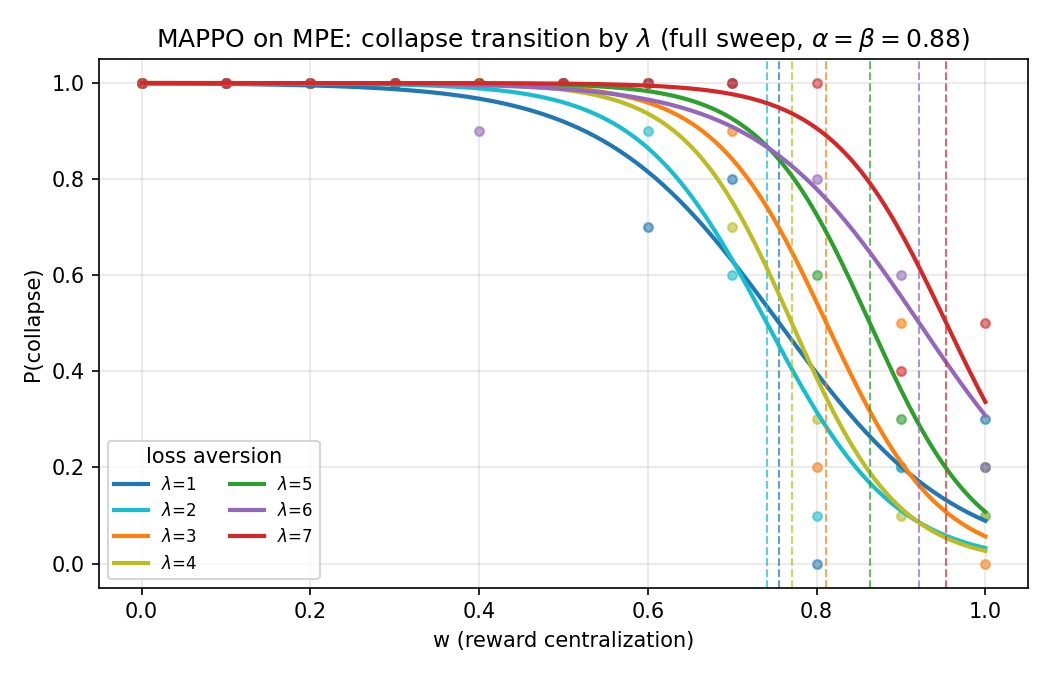
\includegraphics[width=0.92\linewidth]{../docs/expMAPPO_mpe_figures/mappo_mpe_lambda_curves.png}
  \caption{%
    MAPPO on MPE Cooperative Navigation: fitted collapse-probability curves
    $P(\mathrm{collapse}\mid w)$ for the full loss-aversion sweep
    $\lambda{=}1,\ldots,7$ ($\alpha{=}\beta{=}0.88$, centralized critic, 50-step
    horizon, 10 seeds per cell; collapse = per-step landmark occupancy below the
    calibrated $\theta{=}0.164$). The family shifts rightward as $\lambda$ grows,
    with vertical dashed $\wcrit$ lines ordered accordingly---the same loss-aversion
    signature found in the supply chain, recovered under a different environment
    and a different (centralized-critic) algorithm.}
  \label{fig:mpe_lambda_curves}
\end{figure}

\subsection{Across algorithms: MAPPO on the supply chain}
\label{sec:appendix_crossalgo}

The MPE result varies the environment \emph{and} the algorithm at once. To
isolate the algorithm, we re-run the full loss-aversion sweep on the
\emph{identical} supply-chain substrate, grid, seeds, collapse label, and
hyperparameters, changing only the learner from independent PPO to
centralized-critic MAPPO~\citep{yu2022surprising} (700 runs;
$\lambda\in\{1,\ldots,7\}$, $\alpha{=}\beta{=}0.88$, 5 values of $w$, 20 seeds).
The actor consumes only its local observation; the critic consumes the joint
state (CTDE). This isolates the effect of credit assignment from the behavioural
incentive.

The loss-aversion law replicates under MAPPO. The critical centralization rises
with loss aversion from $\wcrit{=}0.796$ $[0.742, 0.860]$ at $\lambda{=}1$ to
$\wcrit{=}0.889$ $[0.856, 0.917]$ at $\lambda{=}7$, monotone from $\lambda{=}2$
onward ($0.747, 0.795, 0.800, 0.851, 0.861, 0.889$) and with non-overlapping
$\lambda{=}1$ vs $\lambda{=}7$ confidence intervals
(\Cref{fig:mappo_curves}; cross-setting summary in \Cref{fig:generalization}). As in
MPE, the \emph{direction} generalizes while the absolute level does not: the MAPPO
boundary sits above the PPO boundary at low $\lambda$ (most visibly the
$\lambda{=}1$ point, $0.796$ vs $0.586$), where MAPPO's transition is shallow and
the $\wcrit$ estimate correspondingly noisier; the two boundaries converge by
$\lambda{\geq}4$ ($|\Delta\wcrit|\leq 0.04$). We therefore report the
loss-aversion direction and monotonicity as algorithm-independent on this
substrate, and the absolute $\wcrit$ (especially at low $\lambda$) as
algorithm-dependent.

\begin{figure}[tbp]
  \centering
  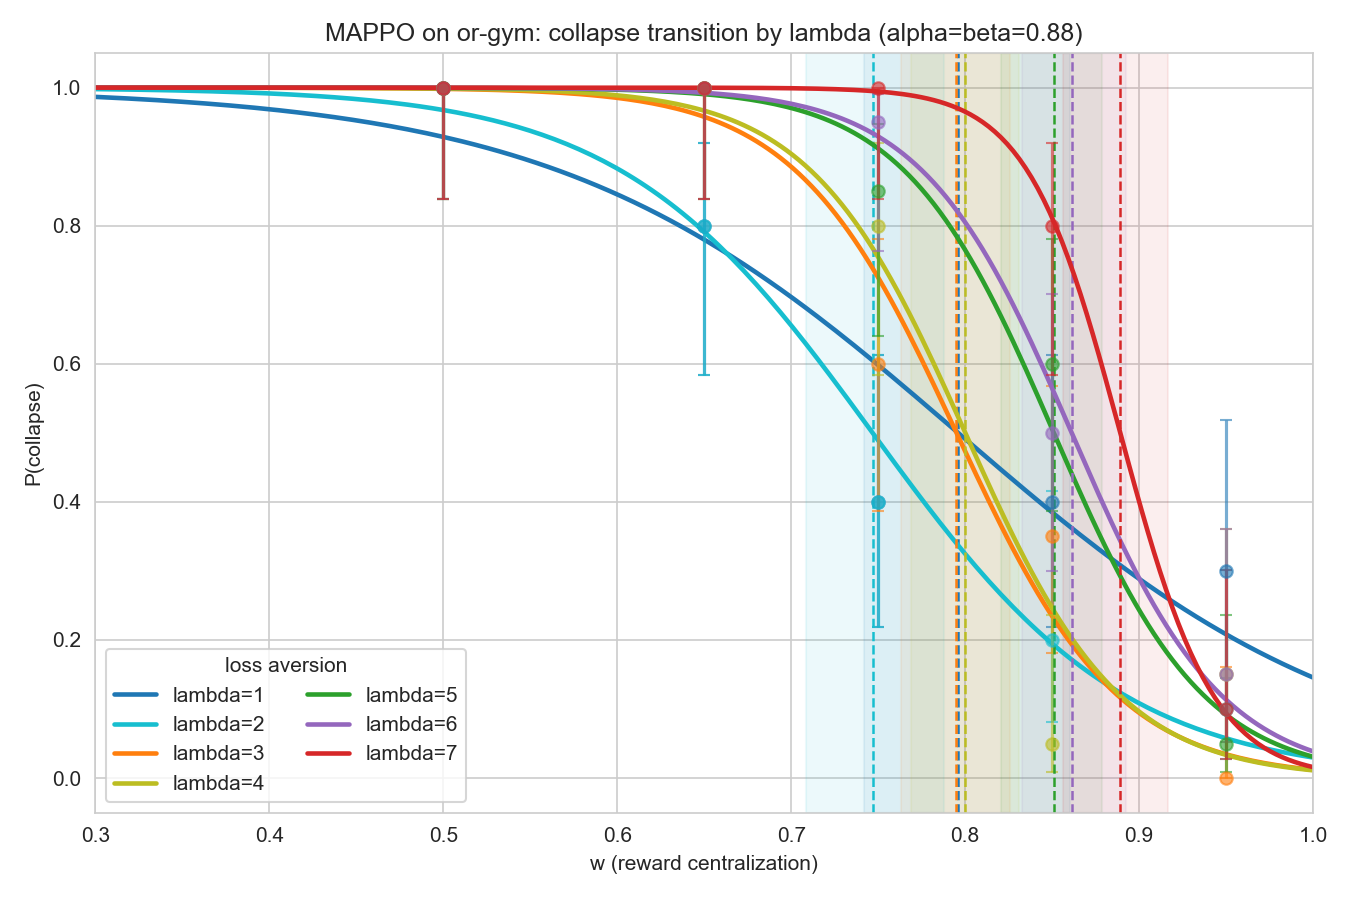
\includegraphics[width=0.82\linewidth]{../docs/expMAPPO_orgym_figures/mappo_orgym_collapse_curves.png}
  \caption{%
    Centralized-critic MAPPO on the supply chain: fitted collapse-probability
    curves $P(\mathrm{collapse}\mid w)$ for $\lambda=1,\ldots,7$
    ($\alpha{=}\beta{=}0.88$, 300k steps, 20 seeds per cell, 700 runs). As under
    PPO, the family shifts rightward as loss aversion grows---each increment of
    $\lambda$ raises the centralization required to avert collapse---confirming
    the effect is not an artifact of independent PPO. The PPO-vs-MAPPO
    $\wcrit(\lambda)$ comparison is shown alongside MPE in
    \Cref{fig:generalization}.}
  \label{fig:mappo_curves}
\end{figure}


% -----------------------------------------------------------------------
\section{Discussion}
\label{sec:discussion}

% D1: the opposite-effects finding is the main result
The finding that probability weighting and loss aversion exert opposite
effects on the coordination boundary is, to our knowledge, novel.
Prior work applies prospect theory as a unified behavioural model without
decomposing its components~\citep{lalmohammed2025,ghaemi2024risk}.
Our null-model design isolates the two components, revealing that the
beneficial effect of curvature ($-0.100$) is masked when combined with
loss aversion ($\lambda{>}1$), which reverses the sign and amplifies the
required centralization.
This has a concrete operational interpretation: a system with $\lambda{=}7$
agents---calibrated to reflect human loss aversion
estimates~\citep{tversky1992}---requires $w > 0.851$ for reliable
coordination, compared to $w > 0.666$ for risk-neutral agents.
The additional 16.6 percentage points of centralization attributable to
behavioral bias ($\wcrit(\lambda{=}7) - \wcrit(\text{null}) =
0.851 - 0.685 = 0.166$, consistent with the excess in
\Cref{tab:decomposition}) are a quantified cost of deploying loss-averse
agents in a cooperative system.

% D1b: heterogeneous minority -- promoted to a main result
The shift is not an averaged, population-wide property: it is driven by a
minority, and by network position. A single \emph{downstream} loss-averse
node ($\lambda{=}7$ at the most demand-facing learning node) moves the
system boundary to $\wcrit = 0.853$, matching a fully loss-averse
population ($0.851$), whereas the same node placed upstream reaches only
$0.726$ (Section~\ref{sec:appendix_robustness2}). Loss aversion therefore cascades
\emph{upstream}---a downstream node's bias propagates back along the
ordering chain and dominates the system boundary---but not downstream, a
directional asymmetry that mirrors the bullwhip structure of the substrate.
That a behavioral minority can move a system-level tipping point is itself
established in evolutionary game theory via replicator
selection~\citep{mengesha2025}; our contribution is the deep-MARL
instantiation, where the effect emerges from gradient learning dynamics and
carries a concrete network-position signature absent from the EGT account.
The operational reading is sharper than a population average would suggest:
in a mixed human--agent supply chain, the centralization a system needs is
set by its most downstream loss-averse participant, not by the mean bias.

% D2: metastability -- lazy agent attractor is escapable
The sliding $\wcrit$ result is a positive finding, not a pathology.
It establishes that the lazy-agent attractor is \emph{metastable}: agents
caught below the isocline at finite $T$ can, in principle, coordinate if
given more training.
This is consistent with \citet{weng2026}'s finding that exploration breaks
cooperation in shared-policy MARL during early training, before
representations converge.
The practical implication is that the minimum $w$ required depends on the
operational training budget: tighter horizons demand higher centralization.

% D3: relation to Yamaguchi 2025
\citet{yamaguchi2025} construct a phase diagram in $(L, \rho)$ space for
IQL, identifying analogous coordinated/fragile/jammed regimes.
Our results complement theirs by demonstrating that the phase structure is
not only a function of environmental complexity but also of the reward
structure ($w$) and agent behavioral parameters ($\lambda$).
Together, these works suggest that MARL coordination exhibits coherent
phase structure across multiple parameter axes.
More broadly, competing-bias tipping points are an established analytic
phenomenon in multiagent dynamics: \citet{capannoli2026phase} prove a metastable
partial-adoption boundary in network opinion dynamics under competing stubbornness
and disruptive biases, with an explicit critical threshold. Our contribution is
the deep-MARL \emph{learning-dynamics} analogue---a boundary set by the
policy-gradient signal-to-noise ratio rather than a fixed update rule---which
situates our phase-diagram framing within a recognised line of multiagent
phase-transition results.

% D4: limitations
Several limitations should be noted.
First, the primary quantitative phase diagram is estimated on a single
environment (NetworkManagement-v1) under PPO. We replicate the collapse boundary
and the \emph{direction} of the loss-aversion effect in a second domain (MPE
Cooperative Navigation) via a full $\lambda{=}1,\ldots,7$ sweep
(Section~\ref{sec:appendix_environments}); because that environment's coordination
reward is shared-global rather than per-agent, independent PPO cannot learn its
coordination end (a credit-assignment, not behavioural, failure), so MPE is
trained with centralised-critic MAPPO. We thus match the algorithm to each
environment's learnability rather than holding it fixed. To isolate the
algorithm from the environment, we additionally re-run the full sweep with
centralised-critic MAPPO on the \emph{same} supply-chain substrate
(Section~\ref{sec:appendix_crossalgo}): the loss-aversion direction and monotonicity
replicate, confirming the effect is not specific to independent PPO. The
curvature sign and the precise affine functional form do not transfer to MPE,
and the absolute $\wcrit$ is algorithm-dependent at low $\lambda$; broader
replication across further algorithms and environments remains future work.
Second, the high-$\lambda$ conditions ($\lambda{=}5,7$) have a steep transition
resolved by a single interior $w$-grid point; we address this with Firth
penalized fits (\Cref{tab:lambda_sweep}), but a finer grid above $w{=}0.85$
would further tighten the high-$\lambda$ confidence intervals.
Third, the metastability result describes finite-horizon behavior; an
asymptotic lower bound on $\wcrit$ is not estimated by our experiments.
Fourth, we fix the demand distribution and lead times; the dependence of
$\wcrit$ on these environmental parameters is unexplored.

% -----------------------------------------------------------------------
\section{Conclusion}
\label{sec:conclusion}

We presented the first quantitative phase diagram of cooperative MARL
coordination collapse, characterising the critical centralization threshold
$\wcrit$ as a function of reward structure, training horizon, and
prospect-theoretic loss aversion.
A three-way null-model decomposition reveals that the two components of
prospect theory---probability weighting and loss aversion---exert
statistically significant effects in opposite directions on the
coordination boundary: the former facilitates coordination by $0.100$;
the latter impedes it by up to $0.166$.
These results provide concrete design constraints for deploying cooperative
MARL in behavioral settings and establish a pre-registered phase-diagram
methodology applicable to any cooperative MARL system.

Natural extensions include replication across further algorithms (QMIX) and
environments (SMAC), upgrading the mean-field account
(Section~\ref{sec:meanfield}) from a calibrated mechanism to a quantitative
prediction of $\wcrit$ via direct measurement of the policy-gradient
signal-to-noise ratio (Section~\ref{sec:appendix_snr}), adaptive centralization
scheduling based on the estimated isocline, and characterization of
heterogeneous-$\lambda$ populations.

% -----------------------------------------------------------------------
% \section*{Acknowledgements}
% \label{sec:ack}
% [To be completed.]

% -----------------------------------------------------------------------

% -----------------------------------------------------------------------
\appendix

\section{Threshold Robustness}
\label{sec:appendix_robustness}

We verify that the collapse definition (\Cref{eq:collapse}) is robust to
perturbation of its thresholds.
We re-estimate $\wcrit$ on Exp~A @300k data under nine variants of the
definition, varying $\bar{S}$ threshold over $\{8, 10, 12\}$ and
$\bar{\pi}$ threshold over $\{-102.5, -127.1, -152.5\}$.
Three variants with threshold $\bar{\pi} \leq -152.5$ are degenerate
(the minimum profit in the dataset is $-128.1$, so no run satisfies
this condition); they are excluded.
Across the remaining six estimable variants, the maximum deviation from
the baseline $\wcrit = 0.666$ is $0.015$, well below the confidence
interval width.
We conclude that the collapse definition is robust to $\pm 20\%$ threshold
perturbation.

% -----------------------------------------------------------------------
\section{Pre-registered Test of the Signal-to-Noise Mechanism}
\label{sec:appendix_snr}

The mean-field account (Section~\ref{sec:meanfield}) calibrates the magnitude of
$\wcrit$ rather than predicting it, because the relevant drift and diffusion
coefficients are properties of the stochastic learning dynamics, not static
quantities of the cost matrix. We pre-register here a direct measurement that
would upgrade the magnitude from calibrated to predicted, and we fix its
analysis before running it.

\paragraph{Observable.} The mean-field model treats the policy's mean
base-stock action $\mu$ as a Langevin variable,
$\mathrm{d}\mu = D(w)\,\mathrm{d}t + \sqrt{2\,\Theta(w)}\,\mathrm{d}W$. During
PPO training we log $\mu$ once per update and, over a fixed early-training
window, estimate the drift $D(w)$ (mean increment) and diffusion $\Theta(w)$
(increment variance / 2), forming $\mathrm{SNR}(w)=D(w)/\sqrt{2\Theta(w)}$.

\paragraph{Prediction and decision rule.} We sweep
$w\in\{0.50,\dots,0.90\}$ at the structural condition
($\alpha{=}\beta{=}1,\lambda{=}1$), $20$ seeds per $w$, $150$k steps, and
compare against the \emph{matched-horizon} boundary $\wcrit=0.822$
(Section~\ref{sec:results_structural}). The mechanism is corroborated iff the
measured signal-to-noise crossing's bootstrap $95\%$ CI contains $0.822$.

\paragraph{Outcome.} The result is mixed, and we report it in full. The
\emph{collapse-fraction} of this independent sweep crosses $0.5$ at
$w=0.82$, reproducing the matched-horizon boundary almost exactly---a
positive robustness check on the boundary itself. The \emph{drift-sign}
observable, however, was \emph{inconclusive}: the restoring drift in the
contested band is weakly positive across all $w$ with no genuine
zero-crossing, so it does not localise $\wcrit$. The reason is basin
geometry: PPO initialises above the cooperative optimum ($S{\approx}250$ vs
$S{\approx}150$), and collapses often plunge through the contested band too
quickly to be sampled, biasing the conditioned drift toward survivors. We
therefore do \emph{not} claim a magnitude-level prediction; the boundary
magnitude remains calibrated, as stated in \Cref{tab:ledger}. The mechanism
section stands on its sign-level and functional-form predictions, which are
unaffected. The driver and analysis (with the decision rule encoded) are
released with the code so the test can be re-run with alternative
observables (e.g.\ a longer horizon matched to $\wcrit=0.666$, or a
basin-flow statistic).

% -----------------------------------------------------------------------
\section{Robustness: Exploration Noise and Heterogeneous Populations}
\label{sec:appendix_robustness2}

Two further pre-registered experiments probe the boundary along axes the main
analysis holds fixed: the exploration noise of the learner, and the homogeneity
of the population. Both reuse the identical substrate, PPO configuration, and
collapse label.

\paragraph{Exploration noise (entropy coefficient).}
The mean-field account (Section~\ref{sec:meanfield}) predicts that $\wcrit$ is set by
the signal-to-noise ratio of the policy gradient, so increasing the exploration
term should raise it. We sweep the PPO entropy coefficient at the structural
condition ($\alpha{=}\beta{=}1$, $\lambda{=}1$, 300k, 20 seeds, $w\in\{0.5,
\ldots,0.9\}$). The boundary rises monotonically with exploration noise
(\Cref{fig:entropy}, \Cref{tab:entropy}): $\wcrit = 0.685$ at $\text{ent}{=}0$
(reproducing the null baseline exactly), $0.690$ at $0.001$, $0.715$ at $0.01$,
and beyond $0.05$ the system collapses at \emph{every} tested $w$
($\wcrit$ extrapolates above $1$). This is direct empirical support for the
signal-to-noise mechanism: the location of the boundary is not a function of the
behavioral bias alone but also of the exploration noise that competes with the
diluted cooperative signal, exactly as \eqref{eq:snr} predicts.

\begin{table}[h]
\centering
\caption{Entropy-coefficient ablation ($\alpha{=}\beta{=}1$, $\lambda{=}1$,
300k, 20 seeds/cell). $\wcrit$ with bootstrap 95\% CIs.}
\label{tab:entropy}
\small
\begin{tabular}{cc}
\toprule
entropy coef. & $\wcrit$ (95\% CI) \\
\midrule
0.000 & 0.685 [0.656, 0.710] \\
0.001 & 0.690 [0.667, 0.715] \\
0.010 & 0.715 [0.689, 0.743] \\
0.050 & $>1$ (collapse at all $w$) \\
\bottomrule
\end{tabular}
\end{table}

\begin{figure}[h]
  \centering
  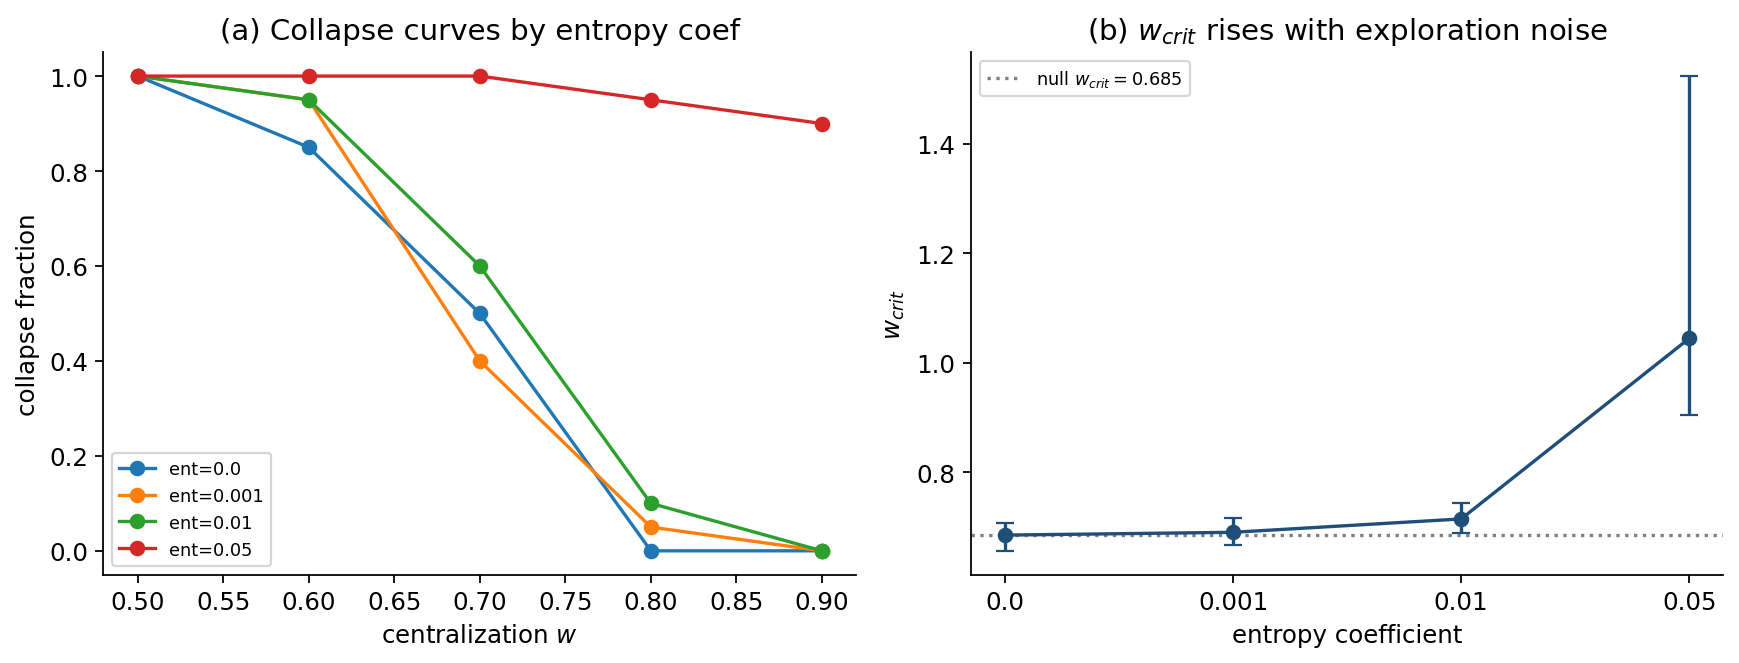
\includegraphics[width=\linewidth]{../docs/expEnt_figures/entropy_ablation.png}
  \caption{Exploration-noise ablation. (a)~Collapse curves shift right as the
  entropy coefficient grows. (b)~$\wcrit$ rises monotonically with exploration
  noise, corroborating the signal-to-noise mechanism (Section~\ref{sec:meanfield});
  $\text{ent}{=}0$ reproduces the null boundary $0.685$.}
  \label{fig:entropy}
\end{figure}

\paragraph{Heterogeneous cognitive profiles.}
We next ask whether a single loss-averse node destabilises an otherwise
risk-neutral network, and whether its network position matters. We assign
$\lambda{=}7$ to selected nodes and $\lambda{=}1$ to the rest
($\alpha{=}\beta{=}0.88$, 300k, 20 seeds, $w\in\{0.5,0.65,0.75,0.85,0.95\}$).
The effect is large and strongly position-dependent (\Cref{fig:hetero},
\Cref{tab:hetero}). A single \emph{downstream} loss-averse node drives
$\wcrit = 0.853$ $[0.849,0.858]$---statistically indistinguishable from the
\emph{fully} loss-averse population ($\wcrit = 0.851$ $[0.847,0.856]$): one
irrational node downstream poisons the entire network. A single \emph{upstream}
loss-averse node shifts the boundary far less, to $\wcrit = 0.726$
$[0.689,0.763]$. Loss aversion therefore cascades upstream---a downstream
node's bias propagates through the ordering chain and dominates the system
boundary---but does not cascade downstream, a directional asymmetry consistent
with the bullwhip structure of the substrate. The practical implication is
sharp: in a mixed human--agent supply chain, the system-level centralization
requirement is governed by the most downstream loss-averse participant, not by
the population average.

\begin{table}[h]
\centering
\caption{Heterogeneous-population sweep ($\alpha{=}\beta{=}0.88$; loss-averse
nodes at $\lambda{=}7$, others $\lambda{=}1$; 300k, 20 seeds/cell).
$\wcrit$ with bootstrap 95\% CIs. Homogeneous references: all risk-neutral
$\approx 0.586$, all loss-averse $0.851$.}
\label{tab:hetero}
\small
\begin{tabular}{lc}
\toprule
Loss-averse nodes & $\wcrit$ (95\% CI) \\
\midrule
one upstream                   & 0.726 [0.689, 0.763] \\
one downstream                 & 0.853 [0.849, 0.858] \\
two downstream                 & 0.851 [0.847, 0.856] \\
all five (homogeneous)         & 0.851 [0.847, 0.856] \\
\bottomrule
\end{tabular}
\end{table}

\begin{figure}[h]
  \centering
  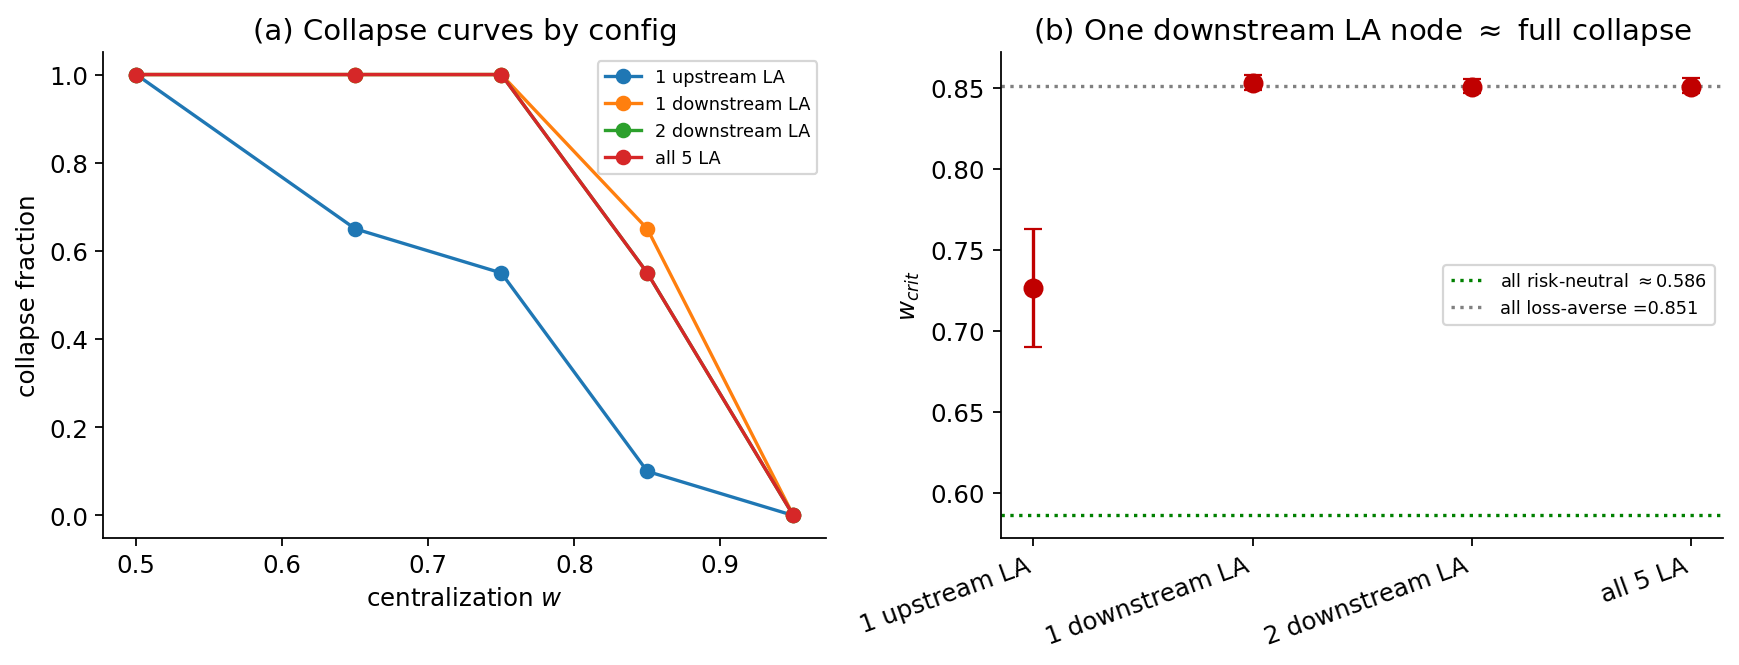
\includegraphics[width=\linewidth]{../docs/expHet_figures/heterogeneous.png}
  \caption{Heterogeneous cognitive profiles. (a)~Collapse curves: a single
  downstream loss-averse node (orange) tracks the fully loss-averse population
  (red), while a single upstream node (blue) is far milder. (b)~$\wcrit$ by
  configuration: one downstream loss-averse node already reaches the homogeneous
  loss-averse boundary; loss aversion cascades upstream but not downstream.}
  \label{fig:hetero}
\end{figure}

% -----------------------------------------------------------------------
\bibliographystyle{plainnat}
\bibliography{references_aaai}

\end{document}